\documentclass{article}




\usepackage{fullpage}
\usepackage{nopageno}
\usepackage{amsmath}
\usepackage{amsfonts}
\usepackage{graphicx}
\usepackage{framed}
\usepackage{algorithmic}
\usepackage{xcolor}

\definecolor{dark_red}{rgb}{0.5,0.0,0.0}
\definecolor{dark_green}{rgb}{0.0,0.5,0.0}
\definecolor{dark_blue}{rgb}{0.0,0.0,0.5}
\definecolor{blue}{rgb}{0.0,0.0,1.0}

\newcommand{\dr}[1]{\textcolor{dark_red}{#1}}
\newcommand{\dg}[1]{\textcolor{dark_green}{#1}}
\newcommand{\db}[1]{\textcolor{dark_blue}{#1}}
\newcommand{\blue}[1]{\textcolor{blue}{#1}}


\usepackage{fancyhdr}
%\setlength{\footheight}{15.2pt}
\pagestyle{fancy}
\fancyhead[C]{Wentworth Institute of Technology, MATH2025}
\fancyfoot[C]{Author: Shawn Eastwood}
\renewcommand{\headsep}{25pt}
\renewcommand{\headrulewidth}{1pt}
\renewcommand{\footrulewidth}{1pt}


\begin{document}


\subsection*{Vectors with an arbitrary number of dimensions: a review}

{\bf Vectors do not necessarily have \(3\) components.} With an arbitrary natural number \(n\) an ``\(n\)-component vector" is simply a list of \(n\) numbers:
\[\mathbf{u} = \begin{bmatrix} u_1 \\ u_2 \\ \vdots \\ u_n \end{bmatrix}\]
also represented by 
\[\mathbf{u} = \langle u_1, u_2, ..., u_n \rangle\]
Math associated with \(n\) component vectors is: 
\begin{itemize}
\item Vector addition:
\[\begin{bmatrix} u_1 \\ u_2 \\ \vdots \\ u_n \end{bmatrix} + \begin{bmatrix} v_1 \\ v_2 \\ \vdots \\ v_n \end{bmatrix} = \begin{bmatrix} u_1 + v_1 \\ u_2 + v_2 \\ \vdots \\ u_n + v_n \end{bmatrix}\]
\item Scalar multiplication:
\[c\begin{bmatrix} u_1 \\ u_2 \\ \vdots \\ u_n \end{bmatrix} = \begin{bmatrix} u_1 \\ u_2 \\ \vdots \\ u_n \end{bmatrix}c = \begin{bmatrix} c u_1 \\ c u_2 \\ \vdots \\ c u_n \end{bmatrix}\]
\item Magnitude:
\[\left\|\begin{bmatrix} u_1 \\ u_2 \\ \vdots \\ u_n \end{bmatrix}\right\| = \sqrt{u_1^2 + u_2^2 + ... + u_n^2}\] 
\item Dot product:
\[\begin{bmatrix} u_1 \\ u_2 \\ \vdots \\ u_n \end{bmatrix} \bullet \begin{bmatrix} v_1 \\ v_2 \\ \vdots \\ v_n \end{bmatrix} = u_1 v_1 + u_2 v_2 + ... + u_n v_n \]
\end{itemize}
The cross product is only defined for \(3\) component vectors.


\section*{Multivariable functions}

Vector valued functions that described parametric curves were functions that accepted as input a single value, the parameter value, and returned as output a list of numbers, the position vector of the generated point. Now will be considered {\bf multivariable functions}, which are functions that take more than 1 parameter, or equivalently a list of parameters, essentially a vector. For now multivariable functions will only return single values, a.k.a. scalars.   

Multivariable functions are denoted by \(f(x_1, x_2, ..., x_n)\) where \(x_1\), \(x_2\), ..., \(x_n\) are the parameters of multivariable function \(f\). 2 variable functions are often denoted by \(f(x,y)\), and 3 variable functions are often denoted by \(f(x,y,z)\). Since vectors are lists of numbers, multivariable functions are often denoted by \(f(\mathbf{q})\) where \(\mathbf{q}\) is a vector whose components are the parameters. 2 variable functions can be denoted by \(f\left(\begin{bmatrix} x \\ y \end{bmatrix}\right)\), and 3 variable functions can be denoted by \(f\left(\begin{bmatrix} x \\ y \\ z \end{bmatrix}\right)\).

\textbf{Examples:}
\begin{itemize}
\item Consider the two parameter function:
\[f\left(\begin{bmatrix} x \\ y \end{bmatrix}\right) = f(x, y) = x^2 + 3y - 4\]
It is then the case that:
\[f\left(\begin{bmatrix} 2 \\ -1 \end{bmatrix}\right) = f(2, -1) = 2^2 + 3(-1) - 4
= 4 - 3 - 4 = -3\]
and
\[f\left(\begin{bmatrix} 3 \\ -4 \end{bmatrix}\right) = f(3, -4) = 3^2 + 3(-4) - 4
= 9 - 12 - 4 = -7\]
\end{itemize}



\subsection*{Domains}

The domain of a multi-variable function \(f(x_1, x_2, ..., x_n)\) is the set of all of \(n\)-tuples (\(n\) entry lists) where \(f(x_1, x_2, ..., x_n)\) is defined. 

\textbf{Examples:}
\begin{itemize} 
%%%%%%%%%%%%%%%%%%%%%%%%%%%%
\item 
\begin{tabular}{cc}
\parbox{0.6\textwidth}{
The domain of the function:
\[f(x, y) = \left(\sqrt{x^2 + 1 - y}\right) - 5\sqrt{7 - y}\]   
is the set of all \((x, y)\) points where \(x^2 + 1 - y \geq 0\) and \(7 - y \geq 0\). These conditions can be rewritten to \(y \leq x^2 + 1\) and \(y \leq 7\). The domain illustrated on the right.
} & \parbox{0.4\textwidth}{
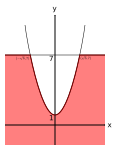
\includegraphics[width = 0.4\textwidth]{two_variable_domain_example_1}
}   
\end{tabular}
%%%%%%%%%%%%%%%%%%%%%%%%%%%%
\item   
The domain of the function:
\[f(x, y, z) = \frac{-3}{1 - y + x - \ln(z)}\]   
is the set of all \((x, y, z)\) points where \(z > 0\) and \(1 - y + x - \ln(z) \neq 0\). 
\end{itemize}



\subsection*{Limits}

Given a multivariable function \(f(x_1, x_2, ..., x_n)\), and a list of input values \((a_1, a_2, ..., a_n)\), then the limit of function \(f(x_1, x_2, ..., x_n)\) as the values of \((x_1, x_2, ..., x_n)\) {\bf simultaneously} approach the respective values of \((a_1, a_2, ..., a_n)\) is denoted by 
\[\lim_{(x_1, x_2, ..., x_n) \rightarrow (a_1, a_2, ..., a_n)} f(x_1, x_2, ..., x_n)\]

The more precise definition is:
\[\lim_{(x_1, x_2, ..., x_n) \rightarrow (a_1, a_2, ..., a_n)} f(x_1, x_2, ..., x_n) = L\]
if and only if for every possible value of \(\epsilon\) where \(\epsilon > 0\), there exists a value of \(\delta\) where \(\delta > 0\) {\bf and}: \\
\begin{itemize}
\item {\bf For every} possible list of parameter values \((x_1, x_2, ..., x_n)\) where: 
	\begin{itemize}
	\item[*] \((x_1, x_2, ..., x_n)\) is within a ``distance" of \(\delta\) of \((a_1, a_2, ..., a_n)\).
	\item[*] \((x_1, x_2, ..., x_n)\) {\bf is not equal to} \((a_1, a_2, ..., a_n)\). 
	\end{itemize}
\item {\bf Then} the value of \(f(x_1, x_2, ..., x_n)\) is within a ``distance" of \(\epsilon\) of \(L\). 
\end{itemize}

This can symbolically be represented via:
\[0 < \left\|\begin{bmatrix} x_1 \\ x_2 \\ \vdots \\ x_n \end{bmatrix} - \begin{bmatrix} a_1 \\ a_2 \\ \vdots \\ a_n \end{bmatrix}\right\| < \delta \implies |f(x_1, x_2, ..., x_n) - L| < \epsilon\]

\vspace{5mm}

If \(n\) parameter functions \(f(x_1, x_2, ..., x_n)\) and \(g(x_1, x_2, ..., x_n)\) are equal everywhere except for \((x_1, x_2, ..., x_n) = (a_1, a_2, ..., a_n)\), then the limits as \((x_1, x_2, ..., x_n)\) approaches \((a_1, a_2, ..., a_n)\) are equal:
\[\lim_{(x_1, x_2, ..., x_n) \rightarrow (a_1, a_2, ..., a_n)} f(x_1, x_2, ..., x_n) = \lim_{(x_1, x_2, ..., x_n) \rightarrow (a_1, a_2, ..., a_n)} g(x_1, x_2, ..., x_n)\]

\vspace{5mm}

A function \(f(x_1, x_2, ..., x_n)\) is {\bf continuous} at a point \((a_1, a_2, ..., a_n)\) from the domain of \(f\) if and only if  
\[\lim_{(x_1, x_2, ..., x_n) \rightarrow (a_1, a_2, ..., a_n)} f(x_1, x_2, ..., x_n) = f(a_1, a_2, ..., a_n)\]
\(f\) is continuous if and only if it is continuous at all points in its domain. Most functions that will be considered are continuous at all points in their domain. 

\vspace{5mm}

\textbf{Property: The limit of a continuous single variable function following a multivariable function:}
\begin{itemize}
\item Let \(f(x_1, x_2, ..., x_n)\) denote an \(n\) parameter function. 
\item Let \(h(u)\) denote a single variable function. 
\item Let \((a_1, a_2, ..., a_n)\) denote an arbitrary list of \(n\) quantities. 
\item Let the limit \(\lim_{(x_1, x_2, ..., x_n) \rightarrow (a_1, a_2, ..., a_n)} f(x_1, x_2, ..., x_n)\) exist and be equal to \(L\). 
\item Let \(h(u)\) be continuous at \(u = L\). 
\item {\bf It is then the case that:}
\[\lim_{(x_1, x_2, ..., x_n) \rightarrow (a_1, a_2, ..., a_n)} h(f(x_1, x_2, ..., x_n)) = h\left(\lim_{(x_1, x_2, ..., x_n) \rightarrow (a_1, a_2, ..., a_n)} f(x_1, x_2, ..., x_n)\right) = h(L)\]
\end{itemize}

Examples of this property in use are:
\begin{itemize}
\item Since the function \(h(u) = u^2\) is continuous, 
\[\lim_{(x, y) \rightarrow (a, b)} \left(f(x, y)^2\right) = \left(\lim_{(x, y) \rightarrow (a, b)} f(x, y)\right)^2\]
\item If \(\lim_{(x, y) \rightarrow (a, b)} f(x, y) > 0\), then since the function \(h(u) = \sqrt{u}\) is continuous for all positive numbers,  
\[\lim_{(x, y) \rightarrow (a, b)} \sqrt{f(x, y)} = \sqrt{\lim_{(x, y) \rightarrow (a, b)} f(x, y)}\]
\item Since the function \(h(u) = \sin(u)\) is continuous, 
\[\lim_{(x, y) \rightarrow (a, b)} \sin(f(x, y)) = \sin\left(\lim_{(x, y) \rightarrow (a, b)} f(x, y)\right)\] 
\item If \(\lim_{(x, y) \rightarrow (a, b)} f(x, y) > 0\), then since the function \(h(u) = \ln(u)\) is continuous for all positive numbers,  
\[\lim_{(x, y) \rightarrow (a, b)} \ln(f(x, y)) = \ln\left(\lim_{(x, y) \rightarrow (a, b)} f(x, y)\right)\]
\end{itemize}

\vspace{5mm}

\textbf{Property: The limit of a continuous multivariable function whose inputs are computed from single variable functions:}
\begin{itemize}
\item Let \(f(x_1, x_2, ..., x_n)\) denote an \(n\) parameter function. 
\item Let \(h_1(t)\), \(h_2(t)\), ..., \(h_n(t)\) denote single variable functions. 
\item Let \(t_0\) denote an arbitrary quantity. 
\item Let the limits \(\lim_{t \rightarrow t_0} h_1(t)\), \(\lim_{t \rightarrow t_0} h_2(t)\), ..., \(\lim_{t \rightarrow t_0} h_n(t)\) all exist and be respectively equal to \(a_1\), \(a_2\), ..., \(a_n\). 
\item Let \(f(x_1, x_2, ..., x_n)\) be continuous at \((x_1, x_2, ..., x_n) = (a_1, a_2, ..., a_n)\). 
\item {\bf It is then the case that:}
\[\lim_{t \rightarrow t_0} f(h_1(t), h_2(t), ..., h_n(t)) = f\left(\lim_{t \rightarrow t_0} h_1(t), \lim_{t \rightarrow t_0} h_2(t), ..., \lim_{t \rightarrow t_0} h_n(t)\right) = f(a_1, a_2, ..., a_n)\] 
\end{itemize}

\vspace{5mm}

Basic identities involving limits include the following. Let \((a_1, a_2, ..., a_n)\) denote an arbitrary list of values for the \(n\) parameters \((x_1, x_2, ..., x_n)\). Let \(f(x_1, x_2, ..., x_n)\) and \(g(x_1, x_2, ..., x_n)\) denote arbitrary \(n\) parameter functions where the limits \(\lim_{(x_1, x_2, ..., x_n) \rightarrow (a_1, a_2, ..., a_n)} f(x_1, x_2, ..., x_n)\) and \(\lim_{(x_1, x_2, ..., x_n) \rightarrow (a_1, a_2, ..., a_n)} g(x_1, x_2, ..., x_n)\) both exist. Let \(c\) denote an arbitrary constant.
\begin{itemize}
%%%%%%%%%
\item
\[\lim_{(x_1, x_2, ..., x_n) \rightarrow (a_1, a_2, ..., a_n)} c = c\]
\item For any \(i = 1, 2, ..., n\):
\[\lim_{(x_1, x_2, ..., x_n) \rightarrow (a_1, a_2, ..., a_n)} x_i = a_i\]
%%%%%%%%%
\item 
\begin{align*}
& \lim_{(x_1, x_2, ..., x_n) \rightarrow (a_1, a_2, ..., a_n)} (f(x_1, x_2, ..., x_n) + g(x_1, x_2, ..., x_n)) \\
& = \lim_{(x_1, x_2, ..., x_n) \rightarrow (a_1, a_2, ..., a_n)} f(x_1, x_2, ..., x_n) + \lim_{(x_1, x_2, ..., x_n) \rightarrow (a_1, a_2, ..., a_n)} g(x_1, x_2, ..., x_n)
\end{align*}
%%%%%%%%%
\item
\begin{align*}
& \lim_{(x_1, x_2, ..., x_n) \rightarrow (a_1, a_2, ..., a_n)} (c \cdot f(x_1, x_2, ..., x_n)) 
= c \cdot\lim_{(x_1, x_2, ..., x_n) \rightarrow (a_1, a_2, ..., a_n)} f(x_1, x_2, ..., x_n) 
\end{align*}
%%%%%%%%%
\item 
\begin{align*}
& \lim_{(x_1, x_2, ..., x_n) \rightarrow (a_1, a_2, ..., a_n)} (f(x_1, x_2, ..., x_n) \cdot g(x_1, x_2, ..., x_n)) \\
& = \left(\lim_{(x_1, x_2, ..., x_n) \rightarrow (a_1, a_2, ..., a_n)} f(x_1, x_2, ..., x_n)\right) \cdot \left(\lim_{(x_1, x_2, ..., x_n) \rightarrow (a_1, a_2, ..., a_n)} g(x_1, x_2, ..., x_n)\right) 
\end{align*}
%%%%%%%%%
\item Provided that \(\lim_{(x_1, x_2, ..., x_n) \rightarrow (a_1, a_2, ..., a_n)} g(x_1, x_2, ..., x_n) \neq 0\), 
\begin{align*}
& \lim_{(x_1, x_2, ..., x_n) \rightarrow (a_1, a_2, ..., a_n)} \frac{f(x_1, x_2, ..., x_n)}{g(x_1, x_2, ..., x_n)} 
= \frac{\lim_{(x_1, x_2, ..., x_n) \rightarrow (a_1, a_2, ..., a_n)} f(x_1, x_2, ..., x_n)}{\lim_{(x_1, x_2, ..., x_n) \rightarrow (a_1, a_2, ..., a_n)} g(x_1, x_2, ..., x_n)} 
\end{align*}
\end{itemize}

\vspace{5mm}

\textbf{Examples:}
\begin{itemize}
%%%%%%%%%%%%%%%%%%%%%%%%%
\item Evaluate \(\lim_{(x, y) \rightarrow (4, 5)} (7x - 6y)\)
\begin{align*}
\lim_{(x, y) \rightarrow (4, 5)} (7x - 6y) 
= & 7\left(\lim_{(x, y) \rightarrow (4, 5)} x\right) - 6\left(\lim_{(x, y) \rightarrow (4, 5)} y\right) 
= 7(4) - 6(5) 
= 28 - 30 
= -2 
\end{align*}
%%%%%%%%%%%%%%%%%%%%%%%%%
\item Evaluate \(\lim_{(x, y) \rightarrow (-2, 1)} \frac{x}{\sqrt{2x^2 + y^2}}\)

To verify as to whether \(\lim_{(x, y) \rightarrow (-2, 1)} \frac{x}{\sqrt{2x^2 + y^2}} = \frac{\lim_{(x, y) \rightarrow (-2, 1)} x}{\lim_{(x, y) \rightarrow (-2, 1)} \sqrt{2x^2 + y^2}}\), the limit of the denominator needs to be computed. 
\begin{align*}
\lim_{(x, y) \rightarrow (-2, 1)} (2x^2 + y^2) = & 2\left(\lim_{(x, y) \rightarrow (-2, 1)} x\right)^2 + \left(\lim_{(x, y) \rightarrow (-2, 1)} y\right)^2 \\ 
= & 2(-2)^2 + 1^2 = 8 + 1 = 9
\end{align*}
The function \(h(u) = \sqrt{u}\) is continuous at \(\lim_{(x, y) \rightarrow (-2, 1)} (2x^2 + y^2) = 9\) so the limit of the denominator is:
\begin{align*}
\lim_{(x, y) \rightarrow (-2, 1)} \sqrt{2x^2 + y^2} = & \sqrt{\lim_{(x, y) \rightarrow (-2, 1)} (2x^2 + y^2)} = \sqrt{9} = 3
\end{align*}

The limit of the denominator is nonzero, so therefore:
\begin{align*}
\lim_{(x, y) \rightarrow (-2, 1)} \frac{x}{\sqrt{2x^2 + y^2}} 
= & \frac{\lim_{(x, y) \rightarrow (-2, 1)} x}{\lim_{(x, y) \rightarrow (-2, 1)} \sqrt{2x^2 + y^2}} 
= \frac{-2}{3} = -\frac{2}{3}  
\end{align*}
%%%%%%%%%%%%%%%%%%%%%%%%%
\item Evaluate \(\lim_{(x, y) \rightarrow (0, 0)} \frac{3x^3 + 6xy^2}{5x^2 + 10y^2}\) 

The limit of the denominator is \(\lim_{(x, y) \rightarrow (0, 0)} (5x^2 + 10y^2) = 5(0)^2 + 10(0)^2 = 0\) so:
\[\lim_{(x, y) \rightarrow (0, 0)} \frac{3x^3 + 6xy^2}{5x^2 + 10y^2} \neq \frac{\lim_{(x, y) \rightarrow (0, 0)} (3x^3 + 6xy^2)}{\lim_{(x, y) \rightarrow (0, 0)} (5x^2 + 10y^2)}\]
The expression \(\frac{3x^3 + 6xy^2}{5x^2 + 10y^2}\) is equal to:
\[\frac{3x^3 + 6xy^2}{5x^2 + 10y^2} = \frac{3x(x^2 + 2y^2)}{5(x^2 + 2y^2)} = \frac{3x}{5}\]
for all \((x, y)\) pairs except for \((x, y) = (0, 0)\). 
Therefore:
\[\lim_{(x, y) \rightarrow (0, 0)} \frac{3x^3 + 6xy^2}{5x^2 + 10y^2} = \lim_{(x, y) \rightarrow (0, 0)} \frac{3x}{5} = 0\]
\end{itemize}

\vspace{5mm}
  
How can limits be proven to not exist? The following property will be used to prove that limits that do not exist, do not exist.
\begin{itemize}
\item Let \(f(x_1, x_2, ..., x_n)\) denote an \(n\) parameter function. 
\item Let \(h_1(t)\), \(h_2(t)\), ..., \(h_n(t)\) denote single variable functions. 
\item Let \(t_0\) denote an arbitrary quantity. 
\item Let the limits \(\lim_{t \rightarrow t_0} h_1(t)\), \(\lim_{t \rightarrow t_0} h_2(t)\), ..., \(\lim_{t \rightarrow t_0} h_n(t)\) all exist and be respectively equal to \(a_1\), \(a_2\), ..., \(a_n\). However, let the vector \(\begin{bmatrix} h_1(t) \\ h_2(t) \\ \vdots \\ h_n(t) \end{bmatrix}\) not actually reach the vector \(\begin{bmatrix} a_1 \\ a_2 \\ \vdots \\ a_n \end{bmatrix}\) when \(t \neq t_0\). 
\item {\bf If} the limit \(\lim_{(x_1, x_2, ..., x_n) \rightarrow (a_1, a_2, ..., a_n)} f(x_1, x_2, ..., x_n)\) exists and is equal to \(L\), {\bf then}
\[\lim_{t \rightarrow t_0} f(h_1(t), h_2(t), ..., h_n(t)) = \lim_{(x_1, x_2, ..., x_n) \rightarrow (a_1, a_2, ..., a_n)} f(x_1, x_2, ..., x_n) = L\] 
\end{itemize}

The limit \(\lim_{(x_1, x_2, ..., x_n) \rightarrow (a_1, a_2, ..., a_n)} f(x_1, x_2, ..., x_n)\) can be computed by finding a parametric curve that passes through the point \((a_1, a_2, ..., a_n)\) and computing the limit of \(f\) along this parametric curve. {\bf If this limit takes on different values depending on the choice of curve, then the limit does not exist.}

\vspace{5mm}

\textbf{Examples:}
\begin{itemize}
%%%%%%%%%%%%%%%%%%%%%%%%%%%%%%%%%%%
\item Consider the limit: 
\[\lim_{(x, y) \rightarrow (-2, 1)} \frac{3x + 6y}{-2x - 4y}\] 
The limit of the denominator is:
\[\lim_{(x, y) \rightarrow (-2, 1)} (-2x - 4y) = -2(-2) - 4(1) = 4 - 4 = 0\] so:
\[\lim_{(x, y) \rightarrow (-2, 1)} \frac{3x + 6y}{-2x - 4y} \neq \frac{\lim_{(x, y) \rightarrow (-2, 1)} (3x + 6y)}{\lim_{(x, y) \rightarrow (-2, 1)} (-2x - 4y)}\] 
Parametric curves that pass through the point \((-2, 1)\) will now be analyzed. Let \(m\) be an arbitrary constant, and consider the parametric line:
\[\left\{\begin{array}{c}
x(t) = -2 + t \\ 
y(t) = 1 + m \cdot t
\end{array}\right.\]
(\(m\) is effectively the slope of this line) \\
This line passes through the point \((-2, 1)\) when \(t = 0\). The limit of \(\frac{3x + 6y}{-2x - 4y}\) as \(t\) approaches \(0\) along the parametric line is:
\begin{align*}
& \lim_{t \rightarrow 0} \frac{3x(t) + 6y(t)}{-2x(t) - 4y(t)} 
= \lim_{t \rightarrow 0} \frac{3(-2 + t) + 6(1 + m \cdot t)}{-2(-2 + t) - 4(1 + m \cdot t)}   
= \lim_{t \rightarrow 0} \frac{(3 + 6m)t}{(-2 - 4m)t} \\  
= & \lim_{t \rightarrow 0} \frac{3(1 + 2m)}{-2(1 + 2m)} 
= \left\{\begin{array}{cc}
-3/2 & (m \neq -1/2) \\ 
\text{undefined} & (m = -1/2)
\end{array}\right.
\end{align*}
This limit depends on \(m\), so therefore the limit \(\lim_{(x, y) \rightarrow (-2, 1)} \frac{3x + 6y}{-2x - 4y}\) does not exist. The limit should not depend on the path taken to approach the point \((-2, 1)\).
%%%%%%%%%%%%%%%%%%%%%%%%%%%%%%%%%%%
\item Consider the limit: 
\[\lim_{(x, y) \rightarrow (0, 0)} \frac{x}{x + y}\] 
The limit of the denominator is:
\[\lim_{(x, y) \rightarrow (0, 0)} (x + y) = 0\] so:  
\[\lim_{(x, y) \rightarrow (0, 0)} \frac{x}{x + y} \neq \frac{\lim_{(x, y) \rightarrow (0, 0)} x}{\lim_{(x, y) \rightarrow (0, 0)} (x + y)}\] 
Parametric curves that pass through the point \((0, 0)\) will now be analyzed. Let \(m\) be an arbitrary constant, and consider the parametric line:
\[\left\{\begin{array}{c}
x(t) = t \\ 
y(t) = m \cdot t
\end{array}\right.\]
(\(m\) is effectively the slope of this line) \\
This line passes through the point \((0, 0)\) when \(t = 0\). The limit of \(\frac{x}{x + y}\) as \(t\) approaches \(0\) along the parametric line is: 
\begin{align*}
& \lim_{t \rightarrow 0} \frac{x(t)}{x(t) + y(t)} 
= \lim_{t \rightarrow 0} \frac{t}{t + m \cdot t} 
= \lim_{t \rightarrow 0} \frac{1}{1 + m}  
= \frac{1}{1 + m}
\end{align*}
This limit depends on \(m\), so therefore the limit \(\lim_{(x, y) \rightarrow (0, 0)} \frac{x}{x + y}\) does not exist. The limit should not depend on the path taken to approach the point \((0, 0)\).
%%%%%%%%%%%%%%%%%%%%%%%%%%%%%%%%%%%
\item Consider the limit: 
\[\lim_{(x, y) \rightarrow (0, 0)} \frac{4x^2}{8x^2 - 4xy + y^2}\] 
The limit of the denominator is:
\[\lim_{(x, y) \rightarrow (0, 0)} (8x^2 - 4xy + y^2) = 0\] so:  
\[\lim_{(x, y) \rightarrow (0, 0)} \frac{4x^2}{8x^2 - 4xy + y^2} \neq \frac{\lim_{(x, y) \rightarrow (0, 0)} 4x^2}{\lim_{(x, y) \rightarrow (0, 0)} (8x^2 - 4xy + y^2)}\] 
Parametric curves that pass through the point \((0, 0)\) will now be analyzed. Let \(m\) be an arbitrary constant, and consider the parametric line:
\[\left\{\begin{array}{c}
x(t) = t \\ 
y(t) = m \cdot t
\end{array}\right.\]
(\(m\) is effectively the slope of this line) \\
This line passes through the point \((0, 0)\) when \(t = 0\). The limit of \(\frac{x}{x + y}\) as \(t\) approaches \(0\) along the parametric line is: 
\begin{align*}
& \lim_{t \rightarrow 0} \frac{4x(t)^2}{8x(t)^2 - 4x(t)y(t) + y(t)^2} 
= \lim_{t \rightarrow 0} \frac{4t^2}{8t^2 - 4t(m \cdot t) + (m \cdot t)^2} 
= \lim_{t \rightarrow 0} \frac{4}{8 - 4m + m^2}  
= \frac{4}{8 - 4m + m^2} 
\end{align*}
This limit depends on \(m\), so therefore the limit \(\lim_{(x, y) \rightarrow (0, 0)} \frac{4x^2}{8x^2 - 4xy + y^2}\) does not exist. The limit should not depend on the path taken to approach the point \((0, 0)\).  
%%%%%%%%%%%%%%%%%%%%%%%%%%%%%%%%%%%
%\item Consider the limit: 
%\[\lim_{(x, y) \rightarrow (0, 0)} \frac{x^2}{2x^2 - 2xy^2 + y^4}\] 
%The limit of the denominator is:
%\[\lim_{(x, y) \rightarrow (0, 0)} (2x^2 - 2xy^2 + y^4) = 0\] so:  
%\[\lim_{(x, y) \rightarrow (0, 0)} \frac{x^2}{2x^2 - 2xy^2 + y^4} \neq \frac{\lim_{(x, y) \rightarrow (0, 0)} x^2}{\lim_{(x, y) \rightarrow (0, 0)} (2x^2 - 2xy^2 + y^4)}\] 
%Parametric curves that pass through the point \((0, 0)\) will now be analyzed. Let \(m\) be an arbitrary constant, and consider the parametric line:
%\[\left\{\begin{array}{c}
%x(t) = t \\ 
%y(t) = m \cdot t
%\end{array}\right.\]
%(\(m\) is effectively the slope of this line) \\
%This line passes through the point \((0, 0)\) when \(t = 0\). The limit of \(\frac{x^2}{2x^2 - 2xy^2 + y^4}\) as \(t\) approaches \(0\) along the parametric line is: 
%\begin{align*}
%& \lim_{t \rightarrow 0} \frac{x(t)^2}{2x(t)^2 - 2x(t)y(t)^2 + y(t)^4}  
%= \lim_{t \rightarrow 0} \frac{t^2}{2t^2 - 2t(m \cdot t)^2 + (m \cdot t)^4} 
%= \lim_{t \rightarrow 0} \frac{1}{2 - 2m^2 t + m^4 t^2}  
%= \frac{1}{2} 
%\end{align*}
%This limit does not depends on \(m\), so approaching the point \((0, 0)\) along any straight line results in the limit \(\frac{1}{2}\). This seems to imply that \(\lim_{(x, y) \rightarrow (0, 0)} \frac{x^2}{2x^2 - 2xy^2 + y^4} = \frac{1}{2}\)
\end{itemize}




\section*{Partial derivatives}

Given a multivariable function \(f(x_1, x_2, ..., x_n)\), the partial derivatives of \(f\) are the derivatives that result from holding all variables constant except for the variable that is being differentiated:

For each \(i = 1, 2, ..., n\), the partial derivative \(\frac{\partial f}{\partial x_i}\) is the derivative that results by holding all variables except for \(x_i\) {\bf constant}, and the computing the derivative by treating \(f\) as function of \(x_i\) alone:
\[\frac{\partial f}{\partial x_i} = \lim_{h \rightarrow 0} \frac{f(..., x_{i-1}, x_i + h, x_{i+1}, ...) - f(..., x_{i-1}, x_i, x_{i+1}, ...)}{h}\] 
Note how the symbol ``\(\partial\)" is used instead of ``\(d\)".

The list of partial derivatives forms an \(n\)-component vector referred to as the ``gradient", and is denoted by \(\nabla f\): 
\[\nabla f = \begin{bmatrix} \partial f / \partial x_1 \\ \partial f / \partial x_2 \\ \vdots \\ \partial f / \partial x_n \end{bmatrix}\]

\textbf{Examples:}
\begin{itemize}
%%%%%%%%%%%%%%%%%%%%%%%%%%%%%%%%%%%
\item Consider the multivariable function:
\[f(x, y) = -2x^2 + 4xy + 5y^2 - 7x + y - 11\]
The partial derivatives are:
\begin{align*}
\frac{\partial f}{\partial x} = & \frac{\partial}{\partial x}(-2x^2 + 4xy + 5y^2 - 7x + y - 11) \\ 
= & \frac{d}{dx}(-2x^2 + (4y)x + 5y^2 - 7x + y - 11) & \text{(treat \(y\) as a fixed constant)} \\ 
= & -4x + 4y + 0 - 7 + 0 - 0 \\
= & -4x + 4y - 7 
\end{align*}
and
\begin{align*}
\frac{\partial f}{\partial y} = & \frac{\partial}{\partial y}(-2x^2 + 4xy + 5y^2 - 7x + y - 11) \\ 
= & \frac{d}{dy}(-2x^2 + (4x)y + 5y^2 - 7x + y - 11) & \text{(treat \(x\) as a fixed constant)} \\ 
= & -0 + 4x + 10y - 0 + 1 - 0 \\
= & 4x + 10y + 1  
\end{align*}
The gradient is therefore:
\[\nabla f = \begin{bmatrix}
\partial f/\partial x \\ 
\partial f/\partial y \end{bmatrix} = \begin{bmatrix}
-4x + 4y - 7 \\ 
4x + 10y + 1 
\end{bmatrix}\]
%%%%%%%%%%%%%%%%%%%%%%%%%%%%%%%%%%%
\item Consider the multivariable function:
\[f(x, y, z) = 4xyz - 5y^2 + 3xz + 9\]
The partial derivatives are:
\begin{align*}
\frac{\partial f}{\partial x} = & \frac{\partial}{\partial x}(4xyz - 5y^2 + 3xz + 9) \\ 
= & \frac{d}{dx}((4yz)x - 5y^2 + (3z)x + 9) & \text{(treat \(y\) and \(z\) as fixed constants)} \\ 
= & 4yz - 0 + 3z + 0 \\ 
= & 4yz + 3z 
\end{align*}
and
\begin{align*}
\frac{\partial f}{\partial y} = & \frac{\partial}{\partial y}(4xyz - 5y^2 + 3xz + 9) \\ 
= & \frac{d}{dy}((4xz)y - 5y^2 + 3xz + 9) & \text{(treat \(x\) and \(z\) as fixed constants)} \\ 
= & 4xz - 10y + 0 + 0 \\ 
= & 4xz - 10y 
\end{align*} 
and
\begin{align*}
\frac{\partial f}{\partial z} = & \frac{\partial}{\partial z}(4xyz - 5y^2 + 3xz + 9) \\ 
= & \frac{d}{dz}((4xy)z - 5y^2 + (3x)z + 9) & \text{(treat \(x\) and \(y\) as fixed constants)} \\ 
= & 4xy - 0 + 3x + 0 \\
= & 4xy + 3x
\end{align*} 
The gradient is therefore:
\[\nabla f = \begin{bmatrix}
\partial f/\partial x \\ 
\partial f/\partial y \\
\partial f/\partial z 
\end{bmatrix} = \begin{bmatrix}
4yz + 3z \\ 
4xz - 10y \\ 
4xy + 3x 
\end{bmatrix}\]
%%%%%%%%%%%%%%%%%%%%%%%%%%%%%%%%%%%
\item Consider the multivariable function:
\[f(x, y) = a\cos(2x + y) - a^2\sin(x - y)\]
\(a\) is not a parameter of function \(f(x, y)\), and is simply a constant that represents a number. \\
The partial derivatives are:
\begin{align*}
\frac{\partial f}{\partial x} = & \frac{\partial}{\partial x}(a\cos(2x + y) - a^2\sin(x - y)) \\ 
= & \frac{d}{dx}(a\cos(2x + y) - a^2\sin(x - y)) & \text{(treat \(y\) as a fixed constant)} \\ 
= & -2a\sin(2x + y) - a^2\cos(x - y)
\end{align*}
and 
\begin{align*}
\frac{\partial f}{\partial y} = & \frac{\partial}{\partial y}(a\cos(2x + y) - a^2\sin(x - y)) \\ 
= & \frac{d}{dy}(a\cos(2x + y) - a^2\sin(x - y)) & \text{(treat \(x\) as a fixed constant)} \\ 
= & -a\sin(2x + y) + a^2\cos(x - y)
\end{align*}
The gradient is therefore:
\[\nabla f = \begin{bmatrix}
\partial f/\partial x \\ 
\partial f/\partial y 
\end{bmatrix} = \begin{bmatrix}
-2a\sin(2x + y) - a^2\cos(x - y) \\
-a\sin(2x + y) + a^2\cos(x - y)
\end{bmatrix}\]
\end{itemize}

\vspace{5mm}

The product rule holds for the gradient:

\[\nabla (f(x_1, x_2, ..., x_n) \cdot g(x_1, x_2, ..., x_n)) = (\nabla f) \cdot g(x_1, x_2, ..., x_n) + f(x_1, x_2, ..., x_n) \cdot (\nabla g)\]

\textbf{Examples:}
\begin{itemize}
\item Let \(f(x, y, z)\) and \(g(x, y, z)\) denote two 3 parameter functions. Also let 
\begin{align*}
& f(1, -1, 0) = 5 \quad\quad\text{and}\quad\quad \left.\nabla f \right|_{(1, -1, 0)} = \begin{bmatrix} -7 \\ 1 \\ -9 \end{bmatrix} \\ 
& \text{and}\quad\quad g(1, -1, 0) = -2 \quad\quad\text{and}\quad\quad \left.\nabla g \right|_{(1, -1, 0)} = \begin{bmatrix} 4 \\ -2 \\ 0 \end{bmatrix}
\end{align*}
Using the product rule: 
\begin{align*}
\left.\nabla (f(x, y, z) \cdot g(x, y, z)) \right|_{(1, -1, 0)} = & \left(\left.\nabla f \right|_{(1, -1, 0)}\right) \cdot g(1, -1, 0) + f(1, -1, 0) \cdot \left(\left. \nabla g \right|_{(1, -1, 0)}\right) \\ 
= & \begin{bmatrix} -7 \\ 1 \\ -9 \end{bmatrix} \cdot (-2) + 5 \cdot \begin{bmatrix} 4 \\ -2 \\ 0 \end{bmatrix} 
= \begin{bmatrix} 14 \\ -2 \\ 18 \end{bmatrix} + \begin{bmatrix} 20 \\ -10 \\ 0 \end{bmatrix} 
= \begin{bmatrix} 34 \\ -12 \\ 18 \end{bmatrix}
\end{align*}
\end{itemize}




\subsection*{Higher order partial derivatives}

In an exactly analogous manner to single variable derivatives, higher order partial derivatives are the result of computing the partial derivative of a function that is a partial derivative. Given the \(2\) parameter function \(f(x, y)\), 
\begin{align*}
& \frac{\partial^2 f}{\partial x^2} = \frac{\partial}{\partial x}\left(\frac{\partial f}{\partial x}\right) 
\quad\quad\text{and}\quad\quad
\frac{\partial^2 f}{\partial y \partial x} = \frac{\partial}{\partial y}\left(\frac{\partial f}{\partial x}\right)
\quad\quad\text{and}\quad\quad 
\frac{\partial^2 f}{\partial x \partial y} = \frac{\partial}{\partial x}\left(\frac{\partial f}{\partial y}\right) \\
\quad\quad\text{and}\quad\quad 
& \frac{\partial^2 f}{\partial y^2} = \frac{\partial}{\partial y}\left(\frac{\partial f}{\partial y}\right)
\end{align*}   
The total number of partial derivatives applied to a function is the {\bf order} of the partial derivative. If more than one variable is differentiated, then the partial derivative is referred to as a {\bf mixed partial derivative}.

\vspace{5mm}

\textbf{Examples:}
\begin{itemize}
\item Given the function 
\[f(x, y) = -5x^2 + 7xy + 9y^2 - 11x - 2y + 13\]  
The first order partial derivatives are:
\[\frac{\partial f}{\partial x} = -10x + 7y - 11 \quad\quad\text{and}\quad\quad \frac{\partial f}{\partial y} = 7x + 18y - 2\]  
The second order partial derivatives are: 
\begin{itemize}
\item[*] \(\frac{\partial^2 f}{\partial x^2} = \frac{\partial}{\partial x}\left(\frac{\partial f}{\partial x}\right) = -10\)
\item[*] \(\frac{\partial^2 f}{\partial y \partial x} = \frac{\partial}{\partial y}\left(\frac{\partial f}{\partial x}\right) = 7\)
\item[*] \(\frac{\partial^2 f}{\partial x \partial y} = \frac{\partial}{\partial x}\left(\frac{\partial f}{\partial y}\right) = 7\)
\item[*] \(\frac{\partial^2 f}{\partial y^2} = \frac{\partial}{\partial y}\left(\frac{\partial f}{\partial y}\right) = 18\)   
\end{itemize}
\end{itemize}

\vspace{5mm}

When differentiating by more than one variable, the order in which the differentiation occurs has no effect. Given the \(2\) parameter function \(f(x, y)\), 
\[\frac{\partial^2 f}{\partial y \partial x} = \frac{\partial}{\partial y}\left(\frac{\partial f}{\partial x}\right) = \frac{\partial}{\partial x}\left(\frac{\partial f}{\partial y}\right) = \frac{\partial^2 f}{\partial x \partial y}\]

This can be proven via:
\begin{align*}
\frac{\partial^2 f}{\partial y \partial x} 
= & \frac{\partial}{\partial y}\left(\frac{\partial f}{\partial x}\right) 
= \lim_{h_y \rightarrow 0} \frac{\left.\frac{\partial f}{\partial x}\right|_{(x, y + h_y)} - \left.\frac{\partial f}{\partial x}\right|_{(x, y)}}{h_y} \\  
= & \lim_{h_y \rightarrow 0} \frac{\left(\lim_{h_x \rightarrow 0} \frac{f(x + h_x, y + h_y) - f(x, y + h_y)}{h_x}\right) - \left(\lim_{h_x \rightarrow 0} \frac{f(x + h_x, y) - f(x, y)}{h_x}\right)}{h_y} \\    
= & \lim_{h_y \rightarrow 0} \lim_{h_x \rightarrow 0} \frac{(f(x + h_x, y + h_y) + f(x, y)) - (f(x, y + h_y) + f(x + h_x, y))}{h_x h_y} \\    
= & \lim_{h_x \rightarrow 0} \lim_{h_y \rightarrow 0} \frac{(f(x + h_x, y + h_y) + f(x, y)) - (f(x, y + h_y) + f(x + h_x, y))}{h_x h_y} \\  
= & \lim_{h_x \rightarrow 0} \frac{\left(\lim_{h_y \rightarrow 0} \frac{f(x + h_x, y + h_y) - f(x + h_x, y)}{h_y}\right) - \left(\lim_{h_y \rightarrow 0} \frac{f(x, y + h_y) - f(x, y)}{h_y}\right)}{h_x} \\    
= & \lim_{h_x \rightarrow 0} \frac{\left.\frac{\partial f}{\partial y}\right|_{(x + h_x, y)} - \left.\frac{\partial f}{\partial y}\right|_{(x, y)}}{h_x}   
= \frac{\partial}{\partial x}\left(\frac{\partial f}{\partial y}\right)   
= \frac{\partial^2 f}{\partial x \partial y}
\end{align*}

\textbf{Examples:}
\begin{itemize}
\item Given the function 
\[f(x, y, z) = 6x^3 - 7y^3 + 2z^3 - x^2y + xy^2 - 2x^2z + xz^2 + y^2z - 5yz^2 + 11xyz\]  
The first order partial derivatives are:
\begin{itemize}
\item[*] 
\[\frac{\partial f}{\partial x} = 18x^2 + y^2 + z^2 - 2xy - 4xz + 11yz\]
\item[*]
\[\frac{\partial f}{\partial y} = -x^2 - 21y^2 - 5z^2 + 2xy + 11xz + 2yz\]  
\item[*]
\[\frac{\partial f}{\partial z} =  -2x^2 + y^2 + 6z^2 + 11xy + 2xz - 10yz\]
\end{itemize}
The second order partial derivatives are: 
\begin{itemize}
\item[*]
\[\frac{\partial^2 f}{\partial x^2} = \frac{\partial}{\partial x}\left(\frac{\partial f}{\partial x}\right) = 36x - 2y - 4z\]
\item[*]
\[\frac{\partial^2 f}{\partial y^2} = \frac{\partial}{\partial y}\left(\frac{\partial f}{\partial y}\right) = 2x - 42y + 2z\]
\item[*]
\[\frac{\partial^2 f}{\partial z^2} = \frac{\partial}{\partial z}\left(\frac{\partial f}{\partial z}\right) = 2x - 10y + 12z\]
\item[*]
\[\frac{\partial^2 f}{\partial x \partial y} = \frac{\partial}{\partial x}\left(\frac{\partial f}{\partial y}\right) = \frac{\partial}{\partial y}\left(\frac{\partial f}{\partial x}\right) = -2x + 2y + 11z\]
\item[*]
\[\frac{\partial^2 f}{\partial x \partial z} = \frac{\partial}{\partial x}\left(\frac{\partial f}{\partial z}\right) = \frac{\partial}{\partial z}\left(\frac{\partial f}{\partial x}\right) = -4x + 11y + 2z\]
\item[*]
\[\frac{\partial^2 f}{\partial y \partial z} = \frac{\partial}{\partial y}\left(\frac{\partial f}{\partial z}\right) = \frac{\partial}{\partial z}\left(\frac{\partial f}{\partial y}\right) = 11x + 2y - 10z\]
\end{itemize}
The third order partial derivatives are:
\begin{itemize}
\item[*] 
\[\frac{\partial^3 f}{\partial x^3} = \frac{\partial}{\partial x}\left(\frac{\partial^2 f}{\partial x^2}\right) = 36\] 
\item[*] 
\[\frac{\partial^3 f}{\partial y^3} = \frac{\partial}{\partial y}\left(\frac{\partial^2 f}{\partial y^2}\right) = -42\] 
\item[*]
\[\frac{\partial^3 f}{\partial z^3} = \frac{\partial}{\partial z}\left(\frac{\partial^2 f}{\partial z^2}\right) = 12\]
\item[*]
\[\frac{\partial^3 f}{\partial x^2 \partial y} = \frac{\partial}{\partial y}\left(\frac{\partial^2 f}{\partial x^2}\right) = \frac{\partial}{\partial x}\left(\frac{\partial^2 f}{\partial x \partial y}\right) = -2\]
\item[*] 
\[\frac{\partial^3 f}{\partial x \partial y^2} = \frac{\partial}{\partial x}\left(\frac{\partial^2 f}{\partial y^2}\right) = \frac{\partial}{\partial y}\left(\frac{\partial^2 f}{\partial x \partial y}\right) = 2\]
\item[*]
\[\frac{\partial^3 f}{\partial x^2 \partial z} = \frac{\partial}{\partial z}\left(\frac{\partial^2 f}{\partial x^2}\right) = \frac{\partial}{\partial x}\left(\frac{\partial^2 f}{\partial x \partial z}\right) = -4\]
\item[*] 
\[\frac{\partial^3 f}{\partial x \partial z^2} = \frac{\partial}{\partial x}\left(\frac{\partial^2 f}{\partial z^2}\right) = \frac{\partial}{\partial z}\left(\frac{\partial^2 f}{\partial x \partial z}\right) = 2\]
\item[*]
\[\frac{\partial^3 f}{\partial y^2 \partial z} = \frac{\partial}{\partial z}\left(\frac{\partial^2 f}{\partial y^2}\right) = \frac{\partial}{\partial y}\left(\frac{\partial^2 f}{\partial y \partial z}\right) = 2\]
\item[*] 
\[\frac{\partial^3 f}{\partial y \partial z^2} = \frac{\partial}{\partial y}\left(\frac{\partial^2 f}{\partial z^2}\right) = \frac{\partial}{\partial z}\left(\frac{\partial^2 f}{\partial y \partial z}\right) = -10\]
\item[*]
\[\frac{\partial^3 f}{\partial x \partial y \partial z} = \frac{\partial}{\partial x}\left(\frac{\partial^2 f}{\partial y \partial z}\right) = \frac{\partial}{\partial y}\left(\frac{\partial^2 f}{\partial x \partial z}\right) = \frac{\partial}{\partial z}\left(\frac{\partial^2 f}{\partial x \partial y}\right) = 11\]
\end{itemize}
\end{itemize}




\subsection*{Differentiability and tangent planes} 

With a single variable function \(f(x)\), \(f(x)\) is ``differentiable" at the point \(x = a\) if and only if the derivative \(\frac{df}{dx}\) exists at \(x = a\). When this derivative exists, \(f(x)\) can be approximated for values of \(x\) that are ``close" to \(a\) via the following: 

The definition of the derivative itself implies that the change in \(f\) from \(a\) to \(x\), i. e. \(f(x) - f(a)\), is ``approximately" proportional to the derivative:
\[f(x) - f(a) \approx \left.\frac{df}{dx}\right|_a (x - a)\]
Therefore:
\[f(x) \approx f(a) + \left.\frac{df}{dx}\right|_a (x - a)\]

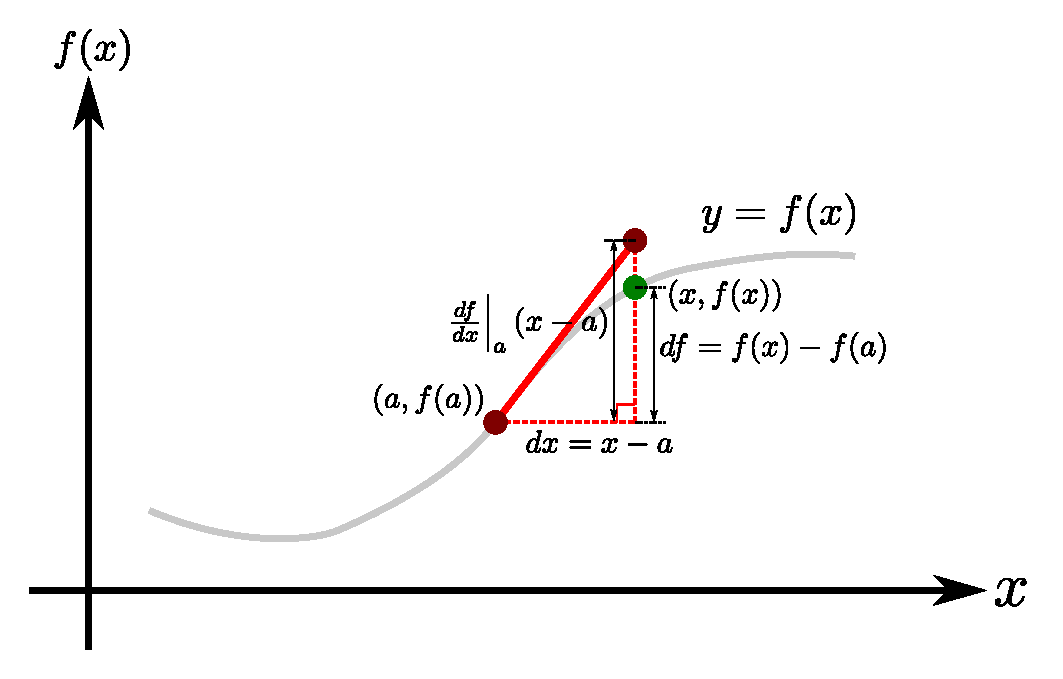
\includegraphics[width = \textwidth]{single_variable_differentiability}

Now this approximation will be generalized to multivariable functions. 

Consider a 2 parameter function \(f(x, y)\). The following discussion will easily generalize to functions with more than 2 parameters.

\(f(x, y)\) is ``differentiable" at the point \((x, y) = (a, b)\) if and only if: 
\begin{itemize}
\item The gradient exists (all of the partial derivatives exist) at the point \((a, b)\).
\item For all points \((x, y)\) that are sufficiently ``close" to \((a, b)\), the approximation 
\[f(x, y) \approx f(a, b) + \left.\frac{\partial f}{\partial x}\right|_{(a, b)} \cdot (x - a) + \left.\frac{\partial f}{\partial y}\right|_{(a,b)} \cdot (y - b)\]
becomes infinitely accurate {\bf relative} to the distance between \((x, y)\) and \((a, b)\).
\end{itemize}
The expression 
\[F_{\text{approx}}(x, y) = f(a, b) + \left.\frac{\partial f}{\partial x}\right|_{(a,b)} \cdot (x - a) + \left.\frac{\partial f}{\partial y}\right|_{(a,b)} \cdot (y - b)\] 
is an approximation for \(f(x, y)\) when \((x, y)\) is ``close" to \((a, b)\).

The term \(\left.\frac{\partial f}{\partial x}\right|_{(a, b)} \cdot (x - a)\) is the approximate increase in \(f(x, y)\) as \(x\) transitions from \(a\) to its current value \(x\).  

The term \(\left.\frac{\partial f}{\partial y}\right|_{(a, b)} \cdot (y - b)\) is the approximate increase in \(f(x, y)\) as \(y\) transitions from \(b\) to its current value \(y\).  

More rigorously: 
\begin{itemize} 
\item The absolute value of difference between the approximation 
\[F_{\text{approx}}(x, y) = f(a, b) + \left.\frac{\partial f}{\partial x}\right|_{(a,b)} \cdot (x - a) + \left.\frac{\partial f}{\partial y}\right|_{(a,b)} \cdot (y - b)\] 
and the true value \(f(x, y)\) is the {\bf absolute error} of the approximation: 
\[\text{absolute-error} = \left|f(x, y) - F_{\text{approx}}(x, y)\right|\]
\item The relative error is the ratio of the absolute error to the distance between the points \((x, y)\) and \((a, b)\):
\[\text{relative-error} = \frac{\text{absolute-error}}{\sqrt{(x - a)^2 + (y - b)^2}}\]
\item The condition for differentiability requires that the relative error diminishes to \(0\) as \((x, y)\) becomes infinitely close to \((a, b)\):
\[\lim_{(x, y) \rightarrow (a, b)} \text{relative-error} = 0\]
\end{itemize}

The approximation \(F_{\text{approx}}(x, y) = f(a, b) + \left.\frac{\partial f}{\partial x}\right|_{(a,b)} \cdot (x - a) + \left.\frac{\partial f}{\partial y}\right|_{(a,b)} \cdot (y - b)\) defines a plane that is tangent to the surface \(z = f(x, y)\) at the point \((a, b, f(a, b))\). The tangent plane has the equation: 
\[z = f(a, b) + \left.\frac{\partial f}{\partial x}\right|_{(a,b)} \cdot (x - a) + \left.\frac{\partial f}{\partial y}\right|_{(a,b)} \cdot (y - b)\] 
This is depicted in the images below:
\begin{center}
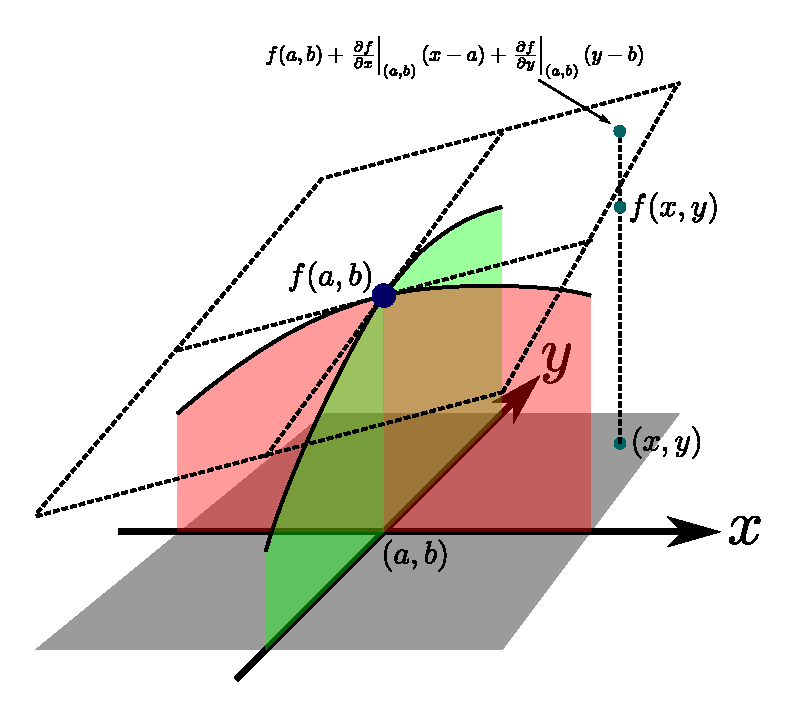
\includegraphics[width = 0.65\textwidth]{differentiability_and_tangent_planes}

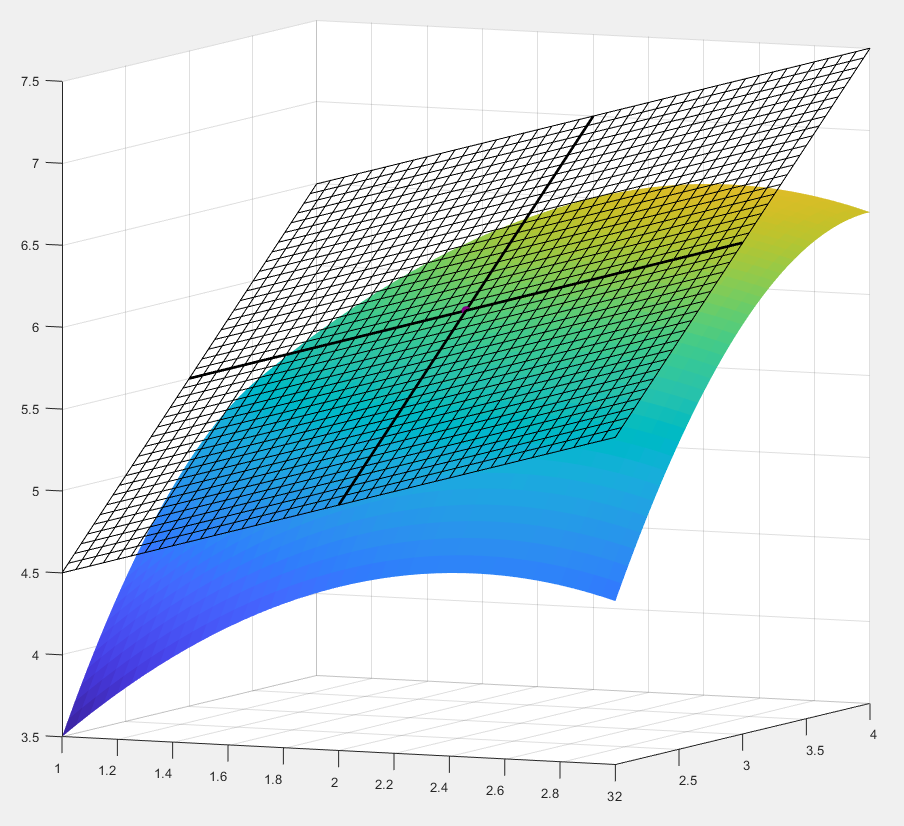
\includegraphics[width = 0.65\textwidth]{differentiability_and_tangent_planes_Matlab.png}
\end{center}

\vspace{5mm}

Unlike for single variable functions, the existence of the partial derivatives does not imply differentiability, meaning that the relative error in the approximation \(f(x, y) \approx f(a, b) + \left.\frac{\partial f}{\partial x}\right|_{(a, b)} \cdot (x - a) + \left.\frac{\partial f}{\partial y}\right|_{(a,b)} \cdot (y - b)\)
 might not diminish to \(0\) as \((x, y)\) gets close to \((a, b)\). As an example of this, consider the function: 
\[f(x,y) = \min(|x|, |y|)\]
and the point \((a, b) = (0, 0)\). Consult the image below: 

\begin{center}
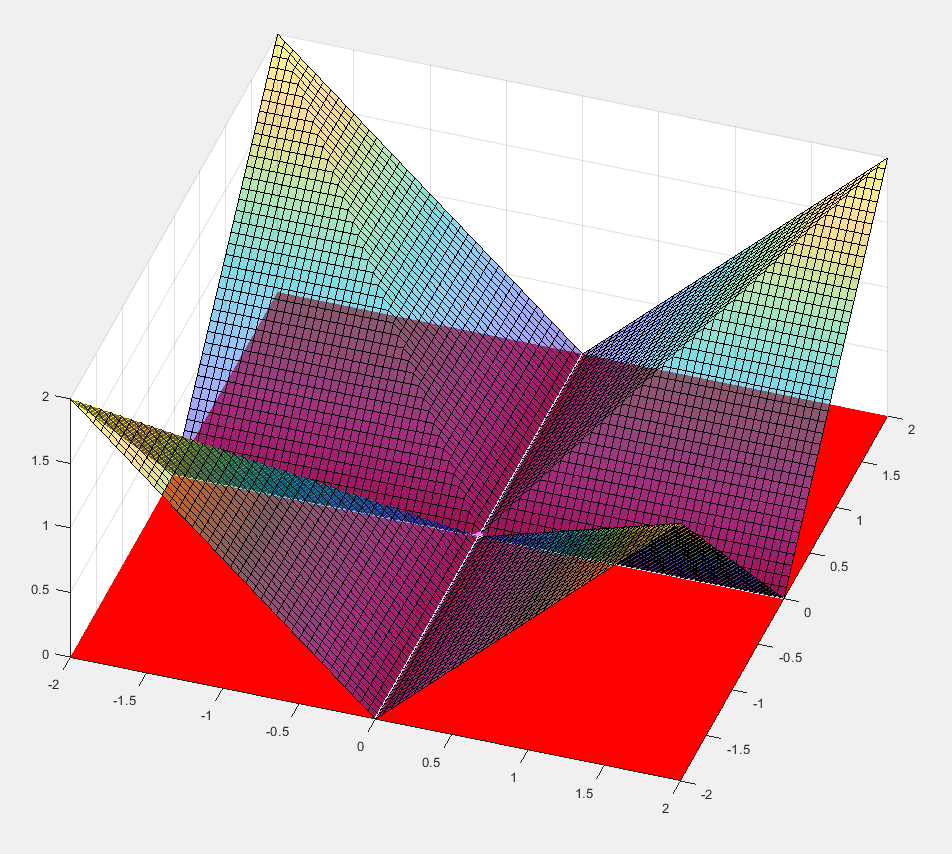
\includegraphics[width = 0.75\textwidth]{non_differentiability_Matlab.png}
\end{center}

At the point \((a, b) = (0, 0)\), the partial derivatives are \(\left.\frac{\partial f}{\partial x}\right|_{(0,0)} = 0\) and \(\left.\frac{\partial f}{\partial y}\right|_{(0,0)} = 0\). The ``approximation" close to \((0, 0)\) is: 
\[F_{\text{approx}}(x, y) = f(0, 0) + \left.\frac{\partial f}{\partial x}\right|_{(0,0)} \cdot (x - 0) + \left.\frac{\partial f}{\partial y}\right|_{(0,0)} \cdot (y - 0) = 0\]
and is denoted by the red plane. It is clear that this is not an accurate approximation due to the folds that are present in the surface. The purpose of this example is to show how a multivariable function may not be differentiable even if the partial derivatives exist.

Most functions considered will be differentiable at all points in their domain.

\vspace{5mm}

\textbf{Examples:}
\begin{itemize}
%%%%%%%%%%%%%%%%%%%%%%%%%%%%%%%%%%%%
\item Consider the two parameter function:
\[f(x, y) = \frac{1}{3}x^3 + 4xy\]
and the input pair \((a, b) = (3, -1)\). The value generated by \(f(a, b)\) is: \(f(3, -1) = 9 - 12 = -3\). 

The plane that is tangent to the surface \(z = \frac{1}{3}x^3 + 4xy\) at the point \((3, -1, f(3, -1)) = (3, -1, -3)\) is what is sought. 

The linear approximation \(F_{\text{approx}}(x, y) = f(a, b) + \left.\frac{\partial f}{\partial x}\right|_{(a,b)} \cdot (x - a) + \left.\frac{\partial f}{\partial y}\right| \cdot (y - b)\) establishes the equation for the desired tangent plane where the value of \(z\) on the tangent plane is \(F_{\text{approx}}(x, y)\). The partial derivatives are: \(\frac{\partial f}{\partial x} = x^2 + 4y\) and \(\frac{\partial f}{\partial y} = 4x\). At the point \((x, y) = (3, -1)\), these partial derivatives are \(\left.\frac{\partial f}{\partial x}\right|_{(3, -1)} = 9 - 4 = 5\) and \(\left.\frac{\partial f}{\partial y}\right|_{(3, -1)} = 12\). The linear approximation becomes:
\begin{align*}
& z = -3 + 5(x - 3) + 12(y + 1) 
\iff z = -3 + (5x - 15) + (12y + 12) 
\iff z = 5x + 12y - 6 
\end{align*}     
The desired tangent plane has the equation:
\[z = 5x + 12y - 6\]
%%%%%%%%%%%%%%%%%%%%%%%%%%%%%%%%%%%%
\item Consider the two parameter function:
\[f(x, y) = x^3 - 2y^2 + 4xy - 9x + 8\]
and the input pair \((a, b) = (1, 2)\). The value generated by \(f(a, b)\) is: \(f(1, 2) = 1 - 8 + 8 - 9 + 8 = -7 - 1 + 8 = 0\). 

The plane that is tangent to the surface \(z = x^3 - 2y^2 + 4xy - 9x + 8\) at the point \((1, 2, f(1, 2)) = (1, 2, 0)\) is what is sought. 

The linear approximation \(F_{\text{approx}}(x, y) = f(a, b) + \left.\frac{\partial f}{\partial x}\right|_{(a,b)} \cdot (x - a) + \left.\frac{\partial f}{\partial y}\right| \cdot (y - b)\) establishes the equation for the desired tangent plane where the value of \(z\) on the tangent plane is \(F_{\text{approx}}(x, y)\). The partial derivatives are: \(\frac{\partial f}{\partial x} = 3x^2 + 4y - 9\) and \(\frac{\partial f}{\partial y} = -4y + 4x\). At the point \((x, y) = (1, 2)\), these partial derivatives are \(\left.\frac{\partial f}{\partial x}\right|_{(1, 2)} = 3 + 8 - 9 = 2\) and \(\left.\frac{\partial f}{\partial y}\right|_{(1, 2)} = -8 + 4 = -4\). The linear approximation becomes:
\begin{align*}
& z = 0 + 2(x - 1) - 4(y - 2) 
\iff z = 0 + (2x - 2) + (-4y + 8) 
\iff z = 2x - 4y + 6 
\end{align*}     
The desired tangent plane has the equation:
\[z = 2x - 4y + 6\]
\end{itemize}



\subsection*{Parallel tangent planes}

Consider an arbitrary surface defined by \(z = f(x, y)\) where \(f(x, y)\) is a 2 parameter function, and a plane with the equation \(z = a x + b y + c\). What is now sought is a point \((x_0, y_0, f(x_0,y_0))\) on the surface where the tangent plane \(z = f(x_0, y_0) + \left.\frac{\partial f}{\partial x}\right|_{(x_0, y_0)} (x - x_0) + \left.\frac{\partial f}{\partial y}\right|_{(x_0, y_0)} (y - y_0)\) is parallel to the plane \(z = a x + b y + c\). For this parallelism to hold, the partial derivatives in the \(x\) and \(y\) directions for the surface and plane must match at \((x, y) = (x_0, y_0)\). It must be the case that \(\left.\frac{\partial f}{\partial x}\right|_{(x_0, y_0)} = a\) and \(\left.\frac{\partial f}{\partial y}\right|_{(x_0, y_0)} = b\). The coordinates \(x_0\) and \(y_0\) must be solved for from this system of 2 equations. The \(z\) coordinate \(f(x_0, y_0)\) is easy to compute.

\vspace{5mm}

\textbf{Examples:}
\begin{itemize}
\item Consider the surface \(z = 3x^2 + 4xy - 5y^2 - 2x + 3y - 9\) and the plane \(z = 8x + 35y + 10\). Let \(f(x, y) = 3x^2 + 4xy - 5y^2 - 2x + 3y - 9\). The point \((x_0, y_0, f(x_0, y_0))\) on the surface \(z = f(x, y)\) where the tangent plane is parallel to the given plane \(z = 8x + 35y + 10\) is sought. 

The partial derivatives are:
\[\frac{\partial f}{\partial x} = 6x + 4y - 2 \quad\quad\text{and}\quad\quad \frac{\partial f}{\partial y} = 4x - 10y + 3\]

The \(x\) and \(y\) coordinates of the desired point, namely \(x_0\) and \(y_0\), must satisfy \(\left.\frac{\partial f}{\partial x}\right|_{(x_0,y_0)} = 8\) and \(\left.\frac{\partial f}{\partial y}\right|_{(x_0,y_0)} = 35\). This gives rise to the system:   
\[\left\{\begin{array}{c}
6x_0 + 4y_0 - 2 = 8 \\ 
4x_0 - 10y_0 + 3 = 35
\end{array}\right.\]
The first equation can be solved to give:
\[6x_0 + 4y_0 - 2 = 8 \iff 4y_0 = 10 - 6x_0 \iff y_0 = \frac{5}{2} - \frac{3}{2}x_0\]
Replacing \(y_0\) in the second equation yields:
\begin{align*}
& 4x_0 - 10(\frac{5}{2} - \frac{3}{2}x_0) + 3 = 35 
\iff 4x_0 + (-25 + 15x_0) + 3 = 35 
\iff 19x_0 = 57 
\iff x_0 = 3 
\end{align*} 
From the value of \(x_0\), 
\[y_0 = \frac{5}{2} - \frac{3}{2}(3) = \frac{-4}{2} = -2\]
With the \(x\) and \(y\) coordinate of the desired point known, the \(z\) coordinate is:
\begin{align*}
f(3, -2) = & 3(3)^2 + 4(3)(-2) - 5(-2)^2 - 2(3) + 3(-2) - 9 \\ 
= & 27 - 24 - 20 - 6 - 6 - 9 
= 3 - 26 - 15 
= -38
\end{align*}
The desired point is:
\[(3, -2, -38)\]
\end{itemize}



\section*{The multi-variable chain rule}

The linear approximation \(F_{\text{approx}}(x, y) = f(a, b) + \left.\frac{\partial f}{\partial x}\right|_{(a,b)} \cdot (x - a) + \left.\frac{\partial f}{\partial y}\right| \cdot (y - b)\) indicates that starting from \((x, y) = (a, b)\), if you change \(x\) by the infinitesimal amount \(dx\) and change \(y\) by the infinitesimal amount \(dy\), the value of \(f(x, y)\) changes in 2 parts: Changing \(x\) from \(a\) by the amount \(dx\) changes \(f(x, y)\) by the amount \(\left.\frac{\partial f}{\partial x}\right|_{(a, b)} dx\). Changing \(y\) from \(b\) by the amount \(dy\) changes \(f(x, y)\) by the amount \(\left.\frac{\partial f}{\partial y}\right|_{(a, b)} dy\). The total change in \(f(x, y)\) is:
\[df = \left.\frac{\partial f}{\partial x}\right|_{(a, b)} dx + \left.\frac{\partial f}{\partial y}\right|_{(a, b)} dy\]
If these changes occur in response to a change in some other value \(t\), then the rates of change with respect to \(t\) are related by:
\[\frac{df}{dt} = \left.\frac{\partial f}{\partial x}\right|_{(a, b)} \frac{dx}{dt} + \left.\frac{\partial f}{\partial y}\right|_{(a, b)} \frac{dy}{dt}\]

To demonstrate the multi-variable chain rule, a series of examples will now be analyzed. Functions that are composed of other functions can be envisioned as flow charts.



\vspace{5mm}

\textbf{Example: the single variable chain rule}

\(f(x)\) and \(g(x)\) are single variable functions. Variable \(t\) is an ``independent" variable, and changes with respect to \(t\) will be computed. Variable \(v = g(f(t))\) is being computed from \(t\). Let \(u = f(t)\) denote the intermediate value as illustrated in the image below:

\begin{center}
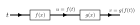
\includegraphics[scale = 1.0]{single_variable_chain_rule}
\end{center}

Initialize \(t\). If \(t\) changes by \(dt\), then \(u\) changes by \(du = \left.\frac{df}{dx}\right|_t dt\). The change in \(u\) then induces in \(v\) a change of \(dv = \left.\frac{dg}{dx}\right|_u du = \left.\frac{dg}{dx}\right|_{f(t)} \left.\frac{df}{dx}\right|_t dt\).

The rate at which \(v\) changes with respect to \(t\) is:
\[\frac{dv}{dt} = \left.\frac{dg}{dx}\right|_{f(t)} \left.\frac{df}{dx}\right|_t\]

As a concrete example, let \(f(x) = x^2 - 5\) and \(g(x) = 3x + 2\). The derivatives of these functions are: \(\frac{df}{dt} = 2x\) and \(\frac{dg}{dt} = 3\). 

Now let \(t = 2\). Next, \(u = f(2) = -1\) and \(v = g(-1) = -1\). The rate of change in \(v\) when \(t = 2\) is sought. The rates of change are \(\left.\frac{df}{dx}\right|_2 = 4\) and \(\left.\frac{dg}{dx}\right|_{-1} = 3\). The rate of change in \(v\) is: 
\[\left.\frac{dv}{dt}\right|_{t = 2} = \left.\frac{dg}{dx}\right|_{-1} \left.\frac{df}{dx}\right|_2 = (3)(4) = 12\]   




\vspace{5mm}

\textbf{Example: the two variable chain rule}

\(f(x)\) and \(g(x)\) are single variable functions. \(h(x, y)\) is a two parameter function. Variable \(t\) is an ``independent" variable, and changes with respect to \(t\) will be computed. Variable \(v = h(f(t), g(t))\) is being computed from \(t\). Let \(u_1 = f(t)\) and \(u_2 = g(t)\) denote the intermediate values as illustrated in the image below:  

\begin{center}
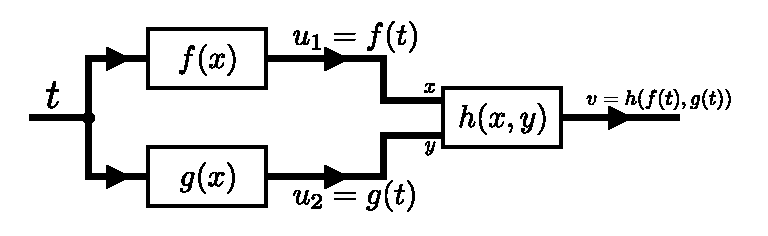
\includegraphics[scale = 1.0]{two_variable_chain_rule}
\end{center}

Initialize \(t\). If \(t\) changes by \(dt\), then \(u_1\) changes by \(du_1 = \left.\frac{df}{dx}\right|_t dt\) and \(u_2\) changes by \(du_2 = \left.\frac{dg}{dx}\right|_t dt\). The changes in \(u_1\) and \(u_2\) both induce a change in \(v\). The total change in \(v\) is: \(dv = \left.\frac{\partial h}{\partial x}\right|_{(u_1, u_2)} du_1 + \left.\frac{\partial h}{\partial y}\right|_{(u_1, u_2)} du_2 = \left.\frac{\partial h}{\partial x}\right|_{(f(t),g(t))} \left.\frac{df}{dx}\right|_t dt + \left.\frac{\partial h}{\partial y}\right|_{(f(t),g(t))} \left.\frac{dg}{dx}\right|_t dt\). The first term comes from the change in \(u_1\), and the second term comes from the change in \(u_2\).  

The rate at which \(v\) changes with respect to \(t\) is:
\[\frac{dv}{dt} = \left.\frac{\partial h}{\partial x}\right|_{(f(t),g(t))} \left.\frac{df}{dx}\right|_t + \left.\frac{\partial h}{\partial y}\right|_{(f(t),g(t))} \left.\frac{dg}{dx}\right|_t\]

As a concrete example, let \(f(x) = 2x\), \(g(x) = x^2\), and \(h(x, y) = \frac{1}{x + y}\). The derivatives of these functions are: \(\frac{df}{dx} = 2\), \(\frac{dg}{dx} = 2x\), \(\frac{\partial h}{\partial x} = \frac{-1}{(x + y)^2}\), and \(\frac{\partial h}{\partial y} = \frac{-1}{(x + y)^2}\). 

Now let \(t = -3\). Next, \(u_1 = f(-3) = -6\), and \(u_2 = g(-3) = 9\), and \(v = h(-6, 9) = \frac{1}{3}\). The rate of change in \(v\) when \(t = -3\) is sought. The rates of change are:
\[\left.\frac{du_1}{dt}\right|_{t = -3} = \left.\frac{df}{dx}\right|_{-3} = 2\]
\[\left.\frac{du_2}{dt}\right|_{t = -3} = \left.\frac{dg}{dx}\right|_{-3} = -6\] 
The rate of change in \(v\) is: 
\[\left.\frac{dv}{dt}\right|_{t = -3} = \left.\frac{\partial h}{\partial x}\right|_{(-6, 9)} \left.\frac{du_1}{dt}\right|_{t = -3} + \left.\frac{\partial h}{\partial y}\right|_{(-6,9)} \left.\frac{du_2}{dt}\right|_{t = -3} = (-\frac{1}{9})(2) + (-\frac{1}{9})(-6) = -\frac{2}{9} + \frac{6}{9} = \frac{4}{9}\]   




\vspace{5mm}

\textbf{Example: the multi-variable chain rule}

\(f_1(x)\), \(f_2(x)\), ..., \(f_n(x)\) are single variable functions. \(h(x_1, x_2, ..., x_n)\) is a \(n\) parameter function. Variable \(t\) is an ``independent" variable, and changes with respect to \(t\) will be computed. Variable \(v = g(f_1(t), f_2(t), ..., f_n(t))\) is being computed from \(t\). Let \(u_1 = f_1(t)\), \(u_2 = f_2(t)\), ..., \(u_n = f_n(t)\) denote the intermediate values as illustrated in the image below:  

\begin{center}
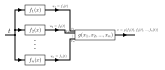
\includegraphics[scale = 1.0]{multi_variable_chain_rule}
\end{center}

Initialize \(t\). If \(t\) changes by \(dt\), then \(u_1\) changes by \(du_1 = \left.\frac{df_1}{dx}\right|_t dt\), \(u_2\) changes by \(du_2 = \left.\frac{df_2}{dx}\right|_t dt\), ..., and \(u_n\) changes by \(du_n = \left.\frac{df_n}{dx}\right|_t dt\). The changes in \(u_1\), \(u_2\), ..., \(u_n\) all induce a change in \(v\). The total change in \(v\) is: \(dv = \left.\frac{\partial g}{\partial x_1}\right|_{(u_1, u_2, ..., u_n)} du_1 + \left.\frac{\partial g}{\partial x_2}\right|_{(u_1, u_2, ..., u_n)} du_2 + ... + \left.\frac{\partial g}{\partial x_x}\right|_{(u_1, u_2, ..., u_n)} du_n = \left.\frac{\partial g}{\partial x_1}\right|_{(f_1(t),f_2(t),...,f_n(t))} \left.\frac{df_1}{dx}\right|_t dt + \left.\frac{\partial g}{\partial x_2}\right|_{(f_1(t),f_2(t),...,f_n(t))} \left.\frac{df_2}{dx}\right|_t dt + ... + \left.\frac{\partial g}{\partial x_n}\right|_{(f_1(t),f_2(t),...,f_n(t))} \left.\frac{df_n}{dx}\right|_t dt\). The first term comes from the change in \(u_1\), and the second term comes from the change in \(u_2\), ..., and the last term comes from the change in \(u_n\).  

The rate at which \(v\) changes with respect to \(t\) is:
\[\frac{dv}{dt} = \left.\frac{\partial g}{\partial x_1}\right|_{(f_1(t),f_2(t),...,f_n(t))} \left.\frac{df_1}{dx}\right|_t + \left.\frac{\partial g}{\partial x_2}\right|_{(f_1(t),f_2(t),...,f_n(t))} \left.\frac{df_2}{dx}\right|_t + ... + \left.\frac{\partial g}{\partial x_n}\right|_{(f_1(t),f_2(t),...,f_n(t))} \left.\frac{df_n}{dx}\right|_t\]



\vspace{5mm}

\textbf{Example: A complex expression}

\(f(x)\), \(g(x)\), and \(h(x)\) are single variable functions. \(a(x, y)\) and \(b(x, y)\) are two parameter functions. Variable \(t\) is an ``independent" variable, and changes with respect to \(t\) will be computed. Variable \(v = b(a(f(t), g(t)), h(t))\) is being computed from \(t\). Let \(u_1 = f(t)\), \(u_2 = g(t)\), \(u_3 = h(t)\), and \(u_4 = a(f(t),g(t))\) denote the intermediate values as illustrated in the image below:  

\begin{center}
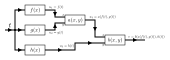
\includegraphics[scale = 1.0]{flow_chart_1}
\end{center}

The rate at which the intermediate values \(u_1\), \(u_2\), and \(u_3\) change with respect to \(t\) are respectively: 

\[\frac{du_1}{dt} = \left.\frac{df}{dx}\right|_t \quad\quad\text{and}\quad\quad \frac{du_2}{dt} = \left.\frac{dg}{dx}\right|_t \quad\quad\text{and}\quad\quad \frac{du_3}{dt} = \left.\frac{dh}{dx}\right|_t\]

The rate at which the intermediate value \(u_4\) changes with respect to \(t\) is:

\[\frac{du_4}{dt} = \left.\frac{\partial a}{\partial x}\right|_{(u_1, u_2)} \frac{du_1}{dt} + \left.\frac{\partial a}{\partial y}\right|_{(u_1, u_2)} \frac{du_2}{dt} 
= \left.\frac{\partial a}{\partial x}\right|_{(f(t), g(t))} \left.\frac{df}{dx}\right|_t + \left.\frac{\partial a}{\partial y}\right|_{(f(t), g(t))} \left.\frac{dg}{dx}\right|_t\]

The rate at which \(v\) changes with respect to \(t\) is:
\begin{align*}
\frac{dv}{dt} = & \left.\frac{\partial b}{\partial x}\right|_{(u_4, u_3)} \frac{du_4}{dt} + \left.\frac{\partial b}{\partial y}\right|_{(u_4, u_3)} \frac{du_3}{dt} \\
= & \left.\frac{\partial b}{\partial x}\right|_{(a(f(t),g(t)), h(t))} \left(\left.\frac{\partial a}{\partial x}\right|_{(f(t), g(t))} \left.\frac{df}{dx}\right|_t + \left.\frac{\partial a}{\partial y}\right|_{(f(t), g(t))} \left.\frac{dg}{dx}\right|_t\right) + \left.\frac{\partial b}{\partial y}\right|_{(a(f(t),g(t)), h(t))} \left.\frac{dh}{dx}\right|_t
\end{align*}

As a concrete example, let \(f(x) = 5x + 1\), and \(g(x) = 3 - x\), and \(h(x) = -2x\), and \(a(x, y) = y - xy\), and \(b(x, y) = x^2 - y^2\). The derivatives of these functions are: \(\frac{df}{dx} = 5\), \(\frac{dg}{dx} = -1\), \(\frac{dh}{dx} = -2\), \(\frac{\partial a}{\partial x} = -y\), \(\frac{\partial a}{\partial y} = 1 - x\), \(\frac{\partial b}{\partial x} = 2x\), and \(\frac{\partial b}{\partial y} = -2y\). 

Now let \(t = 1\). Next, \(u_1 = f(1) = 6\), and \(u_2 = g(1) = 2\), and \(u_3 = h(1) = -2\), and \(u_4 = a(6, 2) = -10\), and \(v = b(-10, -2) = 96\). The rate of change in \(v\) when \(t = 1\) is sought. The rates of change are 
\[\left.\frac{du_1}{dt}\right|_{t = 1} = \left.\frac{df}{dx}\right|_1 = 5\] 
\[\left.\frac{du_2}{dt}\right|_{t = 1} = \left.\frac{dg}{dx}\right|_1 = -1\] 
\[\left.\frac{du_3}{dt}\right|_{t = 1} = \left.\frac{dh}{dx}\right|_1 = -2\]
\[\left.\frac{du_4}{dt}\right|_{t = 1} = \left.\frac{\partial a}{\partial x}\right|_{(6, 2)} \left.\frac{du_1}{dt}\right|_{t = 1} + \left.\frac{\partial a}{\partial y}\right|_{(6, 2)} \left.\frac{du_2}{dt}\right|_{t = 1} = (-2)(5) + (-5)(-1) = -10 + 5 = -5\] 
The rate of change in \(v\) is: 
\[\left.\frac{dv}{dt}\right|_{t = 1} = \left.\frac{\partial b}{\partial x}\right|_{(-10, -2)} \left.\frac{du_4}{dt}\right|_{t = 1} + \left.\frac{\partial b}{\partial y}\right|_{(-10, -2)} \left.\frac{du_3}{dt}\right|_{t = 1} = (-20)(-5) + (4)(-2) = 100 - 8 = 92\]   




\vspace{5mm}

\textbf{Example: Two equivalent inputs}

\(f(x, y)\) is a two variable function. Variable \(t\) is an ``independent" variable, and changes with respect to \(t\) will be computed. Variable \(v = f(t, t)\) is being computed from \(t\).

\begin{center}
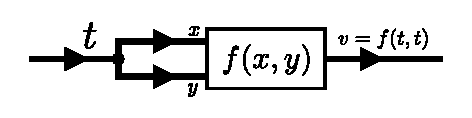
\includegraphics[scale = 1.0]{flow_chart_2}
\end{center}

The rate at which \(v\) changes with respect to \(t\) is:
\begin{align*}
\frac{dv}{dt} = & \left.\frac{\partial f}{\partial x}\right|_{(t, t)} \frac{dt}{dt} + \left.\frac{\partial f}{\partial y}\right|_{(t, t)} \frac{dt}{dt} 
= \left.\frac{\partial f}{\partial x}\right|_{(t, t)} \cdot 1 + \left.\frac{\partial f}{\partial y}\right|_{(t, t)} \cdot 1 \\ 
= & \left.\frac{\partial f}{\partial x}\right|_{(t, t)} + \left.\frac{\partial f}{\partial y}\right|_{(t, t)}  
\end{align*}



\vspace{5mm}

\textbf{Example: Two input and two output variables}

\(f(x, y)\), \(g(x, y)\), \(h(x, y)\), and \(a(x, y)\) are two variable functions. Variables \(t\) and \(s\) are ``independent" variables, and changes with respect to \(t\) and \(s\) will be computed. Variables \(v = h(f(t, s), g(t, s))\) and \(w = a(f(t, s), g(t, s))\) are being computed from \(t\) and \(s\). Let \(u_1 = f(t, s)\), and \(u_2 = g(t, s)\) denote the intermediate values as illustrated in the image below:  

\begin{center}
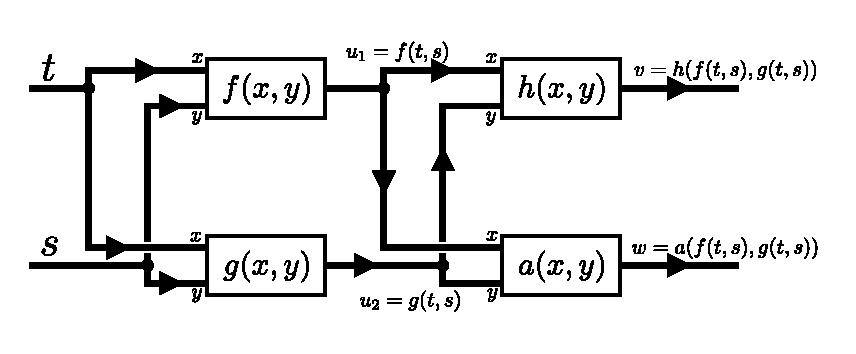
\includegraphics[scale = 1.0]{flow_chart_3}
\end{center}

The rates at which the intermediate value \(u_1\) changes with respect to \(t\) and \(s\) are:

\[\frac{\partial u_1}{\partial t} = \left.\frac{\partial f}{\partial x}\right|_{(t,s)} \quad\quad\text{and}\quad\quad \frac{\partial u_1}{\partial s} = \left.\frac{\partial f}{\partial y}\right|_{(t,s)}\]

The rates at which the intermediate value \(u_2\) changes with respect to \(t\) and \(s\) are:

\[\frac{\partial u_2}{\partial t} = \left.\frac{\partial g}{\partial x}\right|_{(t,s)} \quad\quad\text{and}\quad\quad \frac{\partial u_2}{\partial s} = \left.\frac{\partial g}{\partial y}\right|_{(t,s)}\]

The rates at which \(v\) changes with respect to \(t\) and \(s\) are: 

\[\frac{\partial v}{\partial t} = \left.\frac{\partial h}{\partial x}\right|_{(u_1,u_2)} \frac{\partial u_1}{\partial t} + \left.\frac{\partial h}{\partial y}\right|_{(u_1,u_2)} \frac{\partial u_2}{\partial t} = \left.\frac{\partial h}{\partial x}\right|_{(f(t,s),g(t,s))} \left.\frac{\partial f}{\partial x}\right|_{(t,s)} + \left.\frac{\partial h}{\partial y}\right|_{(f(t,s),g(t,s))} \left.\frac{\partial g}{\partial x}\right|_{(t,s)}\] 
and 
\[\frac{\partial v}{\partial s} = \left.\frac{\partial h}{\partial x}\right|_{(u_1,u_2)} \frac{\partial u_1}{\partial s} + \left.\frac{\partial h}{\partial y}\right|_{(u_1,u_2)} \frac{\partial u_2}{\partial s} = \left.\frac{\partial h}{\partial x}\right|_{(f(t,s),g(t,s))} \left.\frac{\partial f}{\partial y}\right|_{(t,s)} + \left.\frac{\partial h}{\partial y}\right|_{(f(t,s),g(t,s))} \left.\frac{\partial g}{\partial y}\right|_{(t,s)}\] 

The rates at which \(w\) changes with respect to \(t\) and \(s\) are:

\[\frac{\partial w}{\partial t} = \left.\frac{\partial a}{\partial x}\right|_{(u_1,u_2)} \frac{\partial u_1}{\partial t} + \left.\frac{\partial a}{\partial y}\right|_{(u_1,u_2)} \frac{\partial u_2}{\partial t} = \left.\frac{\partial a}{\partial x}\right|_{(f(t,s),g(t,s))} \left.\frac{\partial f}{\partial x}\right|_{(t,s)} + \left.\frac{\partial a}{\partial y}\right|_{(f(t,s),g(t,s))} \left.\frac{\partial g}{\partial x}\right|_{(t,s)}\] 
and 
\[\frac{\partial w}{\partial s} = \left.\frac{\partial a}{\partial x}\right|_{(u_1,u_2)} \frac{\partial u_1}{\partial s} + \left.\frac{\partial a}{\partial y}\right|_{(u_1,u_2)} \frac{\partial u_2}{\partial s} = \left.\frac{\partial a}{\partial x}\right|_{(f(t,s),g(t,s))} \left.\frac{\partial f}{\partial y}\right|_{(t,s)} + \left.\frac{\partial a}{\partial y}\right|_{(f(t,s),g(t,s))} \left.\frac{\partial g}{\partial y}\right|_{(t,s)}\] 




\vspace{5mm}

\textbf{Example: Two inputs, 1 is constant}

\(f(x)\) is a single variable function. \(g(x, y)\) is a two parameter functions. \(c\) is a constant. Variable \(t\) is an ``independent" variable, and changes with respect to \(t\) will be computed. Variable \(v = g(f(t), c)\) is being computed from \(t\). Let \(u_1 = f(t)\) denote the intermediate value as illustrated in the image below:  

\begin{center}
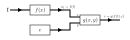
\includegraphics[scale = 1.0]{flow_chart_4}
\end{center}

The rate at which the intermediate value \(u_1\) changes with respect to \(t\) is:

\[\frac{du_1}{dt} = \left.\frac{df}{dx}\right|_t\]

The rate at which \(v\) changes with respect to \(t\) is:
\begin{align*}
\frac{dv}{dt} = & \left.\frac{\partial g}{\partial x}\right|_{(u_1, c)} \frac{du_1}{dt} + \left.\frac{\partial g}{\partial y}\right|_{(u_1, c)} \frac{d}{dt}(c) 
= \left.\frac{\partial g}{\partial x}\right|_{(f(t), c)} \left.\frac{df}{dx}\right|_t + \left.\frac{\partial g}{\partial y}\right|_{(f(t), c)} \cdot 0 
\\
= & \left.\frac{\partial g}{\partial x}\right|_{(f(t), c)} \left.\frac{df}{dx}\right|_t    
\end{align*}
Since the second parameter for \(g(x,y)\) is constant, there is only one component to the rate of change of \(v\) with respect to \(t\).



\subsection*{Directional derivatives and level curves}

Consider a 3 parameter function \(f(x,y,z)\), and associate each triple of input parameters with its corresponding Cartesian coordinate. Given an input point \(\mathbf{q} = \begin{bmatrix} x \\ y \\ z \end{bmatrix}\), the partial derivative \(\frac{\partial f}{\partial x}\) is the rate at which \(f(x, y, z)\) changes when \(\mathbf{q}\) is moved in the positive \(x\) direction, the partial derivative \(\frac{\partial f}{\partial y}\) is the rate at which \(f(x, y, z)\) changes when \(\mathbf{q}\) is moved in the positive \(y\) direction, and the partial derivative \(\frac{\partial f}{\partial z}\) is the rate at which \(f(x, y, z)\) changes when \(\mathbf{q}\) is moved in the positive \(z\) direction. What about other directions? To address this question, let \(\mathbf{q}(t) = \begin{bmatrix} g_x(t) \\ g_y(t) \\ g_z(t) \end{bmatrix}\) describe a parametric curve. Let \(F(t)\) denote the value of \(f(x, y, z)\) at the point \(\mathbf{q}(t)\):
\[F(t) = f(\mathbf{q}(t)) = f(g_x(t), g_y(t), g_z(t))\]

\begin{center}
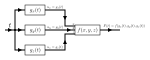
\includegraphics[width = \textwidth]{vector_valued_function_followed_by_3_parameter_function}
\end{center}

Using the multivariable chain rule, the rate at which \(f(x,y,z)\) changes with respect to \(t\) along the parametric curve is:
\begin{align*}
\frac{dF}{dt} = & \left.\frac{\partial f}{\partial x}\right|_{(g_x(t), g_y(t), g_z(t))} \frac{dg_x}{dt} + \left.\frac{\partial f}{\partial y}\right|_{(g_x(t), g_y(t), g_z(t))} \frac{dg_y}{dt} + \left.\frac{\partial f}{\partial z}\right|_{(g_x(t), g_y(t), g_z(t))} \frac{dg_z}{dt} \\
= & \begin{bmatrix} \left.\partial f/\partial x\right|_{\mathbf{q}(t)} \\ \left.\partial f/\partial y\right|_{\mathbf{q}(t)} \\ \left.\partial f/\partial z\right|_{\mathbf{q}(t)} \end{bmatrix} \bullet \begin{bmatrix} dg_x/dt \\ dg_y/dt \\ dg_z/dt \end{bmatrix}
\end{align*}
Recall that the {\bf gradient} is a vector that is a list of the partial derivatives: 
\[\nabla f = \begin{bmatrix} \partial f/\partial x \\ \partial f/\partial y \\ \partial f/\partial z \end{bmatrix}\]
and that the ``velocity" is \(\frac{d\mathbf{q}}{dt} = \begin{bmatrix} dg_x/dt \\ dg_y/dt \\ dg_z/dt \end{bmatrix}\). Therefore:
\[\frac{dF}{dt} = (\nabla f)\Big|_{\mathbf{q}(t)} \bullet \frac{d\mathbf{q}}{dt}\]
The dot product of the gradient and the velocity is the rate at which \(f(x,y,z)\) changes with the parameter \(t\). How about the change with respect to the arc-length \(s\)? Recall that the rate of change in the arc-length distance \(s\) with respect to \(t\) is the speed: \(\frac{ds}{dt} = \left\|\frac{d\mathbf{q}}{dt}\right\|\)
\[\frac{dF}{ds} = \frac{dF/dt}{ds/dt} 
= \frac{(\nabla f)\Big|_{\mathbf{q}(t)} \bullet \frac{d\mathbf{q}}{dt}}{\left\|d\mathbf{q}/dt\right\|} 
= (\nabla f)\Big|_{\mathbf{q}(t)} \bullet \frac{d\mathbf{q}/dt}{\left\|d\mathbf{q}/dt\right\|}\]
The unit length tangent \(\mathbf{T} = \frac{d\mathbf{q}/dt}{\left\|d\mathbf{q}/dt\right\|}\) is a vector with a magnitude of 1 that describes the direction in which the curve is oriented.
\[\frac{dF}{ds} = (\nabla f)\Big|_{\mathbf{q}(t)} \bullet \mathbf{T}\]

If the input point \(\mathbf{q} = \begin{bmatrix} x \\ y \\ z \end{bmatrix}\) moves in a direction described by the {\bf unit magnitude} vector \(\mathbf{T}\), then the rate of change in \(f(x, y, z)\) is the {\bf directional derivative}:
\[\mathbf{T} \bullet (\nabla f)\Big|_{\mathbf{q}}\]

The directional derivative is maximized when \(\mathbf{T}\) points in the direction of the gradient. If \(\mathbf{T} = \frac{\nabla f}{\|\nabla f\|}\), then the directional derivative is at its maximum of \(\frac{\nabla f}{\|\nabla f\|} \bullet (\nabla f) = \frac{\|\nabla f\|^2}{\|\nabla f\|} = \|\nabla f\|\). The unit vector \(\frac{\nabla f}{\|\nabla f\|}\) is the direction of the maximum directional derivative, and the magnitude \(\|\nabla f\|\) is the maximum directional derivative. 

\vspace{5mm}

The directional derivative concept generalizes to multivariable functions with any number of parameters, where there are at least 2 parameters. 


\vspace{5mm}

\textbf{Examples:}
\begin{itemize}
%%%%%%%%%%%%%%%%%%%%%%%%%
\item Let: 
\[f(x,y) = x^3 + x^2 y - y^2 + 2xy + 6\]
At the point \((-1, 1)\), the directional derivative in the direction of \(\mathbf{u} = \begin{bmatrix} -3 \\ 4 \end{bmatrix}\) is sought. 

The unit magnitude vector \(\mathbf{T}\) that has the direction of \(\mathbf{u}\) is:
\[\mathbf{T} = \frac{\mathbf{u}}{\|\mathbf{u}\|} = \begin{bmatrix} -3/5 \\ 4/5 \end{bmatrix}\]

The gradient of \(f(x, y)\) is:
\[\nabla f = \begin{bmatrix} \partial f/\partial x \\ \partial f/\partial y \end{bmatrix}
= \begin{bmatrix}
3x^2 + 2xy + 2y \\ 
x^2 - 2y + 2x 
\end{bmatrix} \quad\quad\text{and}\quad\quad (\nabla f)\Big|_{(-1, 1)} = \begin{bmatrix}
3 - 2 + 2 \\ 
1 - 2 - 2
\end{bmatrix} = \begin{bmatrix}
3 \\ 
-3
\end{bmatrix}\]
The directional derivative is:
\[\mathbf{T} \bullet (\nabla f)\Big|_{(-1, 1)} = -\frac{9}{5} - \frac{12}{5} = -\frac{21}{5}\]
The directional derivatives at the point \((-1, 1)\) has a maximum of 
\[\left\|\nabla f\Big|_{(-1, 1)}\right\| = \sqrt{18} = 3\sqrt{2}\]
and the direction of the maximum directional derivative is
\[\frac{\nabla f\Big|_{(-1, 1)}}{\left\|\nabla f\Big|_{(-1, 1)}\right\|} = \begin{bmatrix}
1/\sqrt{2} \\ 
-1/\sqrt{2} 
\end{bmatrix}\]
%%%%%%%%%%%%%%%%%%%%%%%%%
\item Let: 
\[f(x,y,z) = 4x^3 - x y^2 - 2y + z^2\]
At the point \((0, -2, -1)\), the directional derivative in the direction of \(\mathbf{u} = \begin{bmatrix} -1 \\ 1 \\ 1 \end{bmatrix}\) is sought. 

The unit magnitude vector \(\mathbf{T}\) that has the direction of \(\mathbf{u}\) is:
\[\mathbf{T} = \frac{\mathbf{u}}{\|\mathbf{u}\|} = \begin{bmatrix} -1/\sqrt{3} \\ 1/\sqrt{3} \\ 1/\sqrt{3} \end{bmatrix}\]

The gradient of \(f(x, y, z)\) is:
\[\nabla f = \begin{bmatrix} \partial f/\partial x \\ \partial f/\partial y \\ \partial f/\partial z \end{bmatrix}
= \begin{bmatrix}
12x^2 - y^2 \\ 
-2xy - 2 \\ 
2z
\end{bmatrix} \quad\quad\text{and}\quad\quad (\nabla f)\Big|_{(0, -2, -1)} = \begin{bmatrix}
0 - 4 \\ 
0 - 2 \\ 
-2
\end{bmatrix} = \begin{bmatrix}
-4 \\ 
-2 \\ 
-2 
\end{bmatrix}\]
The directional derivative is:
\[\mathbf{T} \bullet (\nabla f)\Big|_{(0, -2, -1)} 
= \frac{4}{\sqrt{3}} - \frac{2}{\sqrt{3}} - \frac{2}{\sqrt{3}}
= 0\]
The directional derivatives at the point \((0, -2, -1)\) has a maximum of 
\[\left\|\nabla f\Big|_{(0, -2, -1)}\right\| = \sqrt{16 + 4 + 4} = \sqrt{24} = 2\sqrt{6}\]
and the direction of the maximum directional derivative is
\[\frac{\nabla f\Big|_{(0, -2, -1)}}{\left\|\nabla f\Big|_{(0, -2, -1)}\right\|} = \begin{bmatrix}
-2/\sqrt{6} \\ 
-1/\sqrt{6} \\ 
-1/\sqrt{6} 
\end{bmatrix}\]
\end{itemize}




\section*{Level curves and surfaces}

For a two parameter function \(f(x, y)\) a ``level curve" is a curve in the xy-plane where \(f(x, y)\) has the same value at all points along the curve. Given a point \((x_0, y_0)\), the equation \(f(x, y) = f(x_0, y_0)\) is equation of the level curve in the xy-plane that passes through the point \((x_0, y_0)\). 

For a three parameter function \(f(x, y, z)\) a ``level surface" is a surface where \(f(x, y, z)\) has the same value at all points on the surface. Given a point \((x_0, y_0, z_0)\), the equation \(f(x, y, z) = f(x_0, y_0, z_0)\) is equation of the level surface that passes through the point \((x_0, y_0, z_0)\). 

\begin{tabular}{cc}
\parbox{0.5\textwidth}{
At an arbitrary point \(\mathbf{q}_0\), the gradient at \(\mathbf{q}_0\) will always be perpendicular to the level curve/surface that passes through \(\mathbf{q}_0\). This is established by the following reasoning. If unit vector \(\mathbf{T}\) is tangent to the current level curve/surface, then it should be expected that the directional derivative of \(f(\mathbf{q})\) in the direction of \(\mathbf{T}\) is \(0\). This is because \(f(\mathbf{q})\) is constant at all points on the curve/surface. Hence \(\mathbf{T} \bullet (\nabla f)\Big|_{\mathbf{q}_0} = 0\) which means that the gradient \((\nabla f)\Big|_{\mathbf{q}_0}\) will always be perpendicular to \(\mathbf{T}\) so long as \(\mathbf{T}\) is tangent to the level curve/surface. \((\nabla f)\Big|_{\mathbf{q}_0}\) is perpendicular to the level curve/surface.
} & \parbox{0.5\textwidth}{
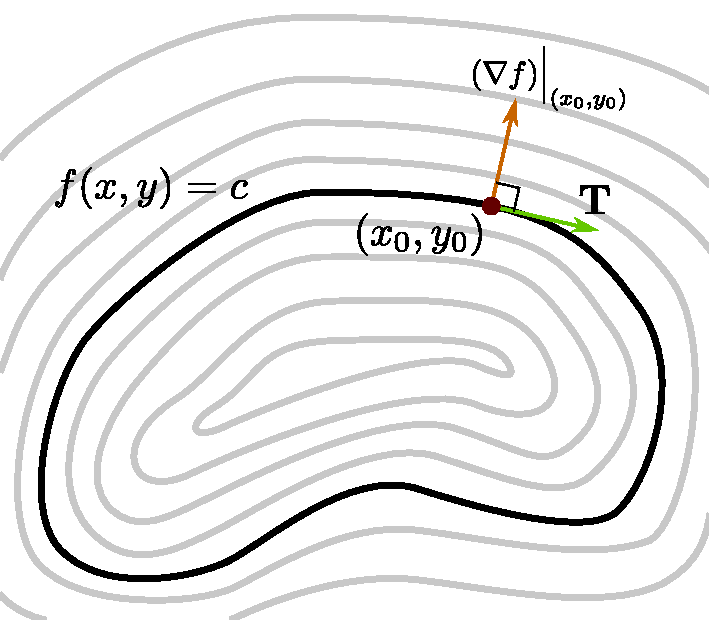
\includegraphics[width = 0.5\textwidth]{level_curves}
}
\end{tabular}

The fact that the gradient vectors will always be perpendicular to the level surfaces of a 3 parameter function can also be used to compute the implicit equation of planes that are tangent to a given surface at a specific point. Consider the surface defined by the equation 
\[f(x,y,z) = c\]
where \(c\) is a constant. This surface is a level surface of \(f(x,y,z)\). Let the point \((x_0, y_0, z_0)\) lie on the surface \(f(x,y,z) = c\) and an implicit equation for the tangent plane that passes through point \((x_0, y_0, z_0)\) is what is sought. The gradient \(\nabla f\Big|_{(x_0, y_0, z_0)}\) is perpendicular to the surface \(f(x,y,z) = c\) and is therefore perpendicular (normal) to the desired tangent plane. The point \((x_0, y_0, z_0)\) lies on the tangent plane, so therefore the equation of the tangent plane is:
\begin{align*}
& \nabla f\Big|_{(x_0, y_0, z_0)} \bullet \begin{bmatrix} x \\ y \\ z \end{bmatrix} = \nabla f\Big|_{(x_0, y_0, z_0)} \bullet \begin{bmatrix} x_0 \\ y_0 \\ z_0 \end{bmatrix}  
\iff \begin{bmatrix} \left.\frac{\partial f}{\partial x}\right|_{(x_0, y_0, z_0)} \\ \left.\frac{\partial f}{\partial y}\right|_{(x_0, y_0, z_0)} \\ \left.\frac{\partial f}{\partial z}\right|_{(x_0, y_0, z_0)} \end{bmatrix} \bullet \begin{bmatrix} x \\ y \\ z \end{bmatrix} = \begin{bmatrix} \left.\frac{\partial f}{\partial x}\right|_{(x_0, y_0, z_0)} \\ \left.\frac{\partial f}{\partial y}\right|_{(x_0, y_0, z_0)} \\ \left.\frac{\partial f}{\partial z}\right|_{(x_0, y_0, z_0)} \end{bmatrix} \bullet \begin{bmatrix} x_0 \\ y_0 \\ z_0 \end{bmatrix} \\ 
& \iff \left.\frac{\partial f}{\partial x}\right|_{(x_0, y_0, z_0)} \cdot x + \left.\frac{\partial f}{\partial y}\right|_{(x_0, y_0, z_0)} \cdot y + \left.\frac{\partial f}{\partial z}\right|_{(x_0, y_0, z_0)} \cdot z \\
& \quad\quad\quad\quad = \left.\frac{\partial f}{\partial x}\right|_{(x_0, y_0, z_0)} \cdot x_0 + \left.\frac{\partial f}{\partial y}\right|_{(x_0, y_0, z_0)} \cdot y_0 + \left.\frac{\partial f}{\partial z}\right|_{(x_0, y_0, z_0)} \cdot z_0 
\end{align*}
This approach also works with the tangent lines of level curves in 2 dimensions.


\textbf{Examples:}
\begin{itemize}
\item Find an implicit equation of the tangent plane to the surface 
\[x^2 - 2xy + 3y^2 + z^2 = 7\]
at the point \((2,1,-2)\). 

Let \(f(x,y,z) = x^2 - 2xy + 3y^2 + z^2\). The gradient is:
\[\nabla f = \begin{bmatrix} \partial f/\partial x \\ \partial f /\partial y \\ \partial f/\partial z \end{bmatrix} = \begin{bmatrix} 2x - 2y \\ -2x + 6y \\ 2z \end{bmatrix}\]
At \((2, 1, -2)\), 
\[\nabla f\Big|_{(2, 1, -2)} = \begin{bmatrix} 2(2) - 2(1) \\ -2(2) + 6(1) \\ 2(-2) \end{bmatrix} = \begin{bmatrix} 4 - 2 \\ -4 + 6 \\ -4 \end{bmatrix} = \begin{bmatrix} 2 \\ 2 \\ -4 \end{bmatrix}\]
This vector is perpendicular to the tangent plane, and is therefore the vector of coefficients of \(x\), \(y\), and \(z\) on the left hand side of the equation of the tangent plane.

The right hand side is: 
\[\nabla f\Big|_{(2, 1, -2)} \bullet \begin{bmatrix} 2 \\ 1 \\ -2 \end{bmatrix} = \begin{bmatrix} 2 \\ 2 \\ -4 \end{bmatrix} \bullet \begin{bmatrix} 2 \\ 1 \\ -2 \end{bmatrix} = 4 + 2 + 8 = 14\]
The equation of the tangent plane is:
\[2x + 2y - 4z = 14\]
\end{itemize}  


\end{document}


























